\documentclass[conference]{IEEEtran}
\IEEEoverridecommandlockouts

\usepackage{cite}
\usepackage{amsmath,amssymb,amsfonts}
\usepackage{algorithmic}
\usepackage{graphicx}
\usepackage{textcomp}
\usepackage{xcolor}
\usepackage{algorithm}
\usepackage{algpseudocode}
\usepackage{tikz}
\usepackage{hyperref}

\def\BibTeX{{\rm B\kern-.05em{\sc i\kern-.025em b}\kern-.08em
    T\kern-.1667em\lower.7ex\hbox{E}\kern-.125emX}}

% Set path for figures
\graphicspath{{Figures/}{report/figures/}}
    
\begin{document}

\title{Playing Flappy Bird Using Deep Reinforcement Learning: A Deep Q-Network Approach\\}

%\author{\IEEEauthorblockN{Manish Murthy}
%\IEEEauthorblockA{\textit{Department of Computer Science} \\
%\textit{University Name}\\
%City, Country \\
%email@university.edu}
%\and
%\IEEEauthorblockN{Sanjana Mandya Lokesh}
%\IEEEauthorblockA{\textit{Department of Computer Science} \\
%\textit{University Name}\\
%City, Country \\
%email@university.edu}
%}

\maketitle

\begin{abstract}
Flappy Bird is a straightforward yet challenging game where players guide a bird through openings between pipes by making it flap its wings. This paper investigates how a reinforcement learning agent can be trained to play Flappy Bird autonomously using Deep Q-Networks (DQN). We demonstrate that by utilizing a compact state representation and a carefully designed reward function, our agent successfully learns an effective policy through experience. Rather than manually coding specific rules, the agent learns optimal behavior through trial and error, determining when to flap and when to glide to maximize its survival time. We detail our implementation approach, including environment construction, neural network architecture, and the impact of various hyperparameters. Our results show that the DQN agent achieves an average score of 15.7 after 5000 training episodes, significantly outperforming random play and approaching skilled human performance. This work illustrates how reinforcement learning techniques originally developed for Atari games can be effectively applied to other dynamic environments and provides insights into the practical challenges of implementing DQN for real-time decision-making tasks.
\end{abstract}

\begin{IEEEkeywords}
Deep Reinforcement Learning, Deep Q-Networks, Flappy Bird, Game AI, Experience Replay, Epsilon-greedy Policy
\end{IEEEkeywords}

% Include each section
\section{Introduction}

Deep reinforcement learning has emerged as a powerful paradigm for training autonomous agents to interact with complex environments. Building upon the foundational principles of reinforcement learning, deep neural networks now enable agents to learn directly from high-dimensional sensory inputs without the need for handcrafted features. This integration has propelled significant advances in artificial intelligence, particularly in domains where designing explicit algorithms remains challenging.

In this paper, we investigate the application of deep reinforcement learning to the Flappy Bird game environment—a deceptively simple yet challenging control task that requires precise timing and decision-making. Flappy Bird presents an interesting case study due to its straightforward mechanics combined with tight constraints on successful navigation. The player controls a bird that must fly between columns of pipes without colliding with them. The game's physics-based dynamics, coupled with the need for precise control, make it an ideal testbed for evaluating reinforcement learning algorithms.

Our work focuses specifically on implementing a Deep Q-Network (DQN) approach, as pioneered by Mnih et al. \cite{mnih2015human} and subsequently refined through numerous innovations in the field. Rather than programming explicit rules for gameplay, we demonstrate how an agent can learn optimal behavior through trial and error, determining when to flap its wings and when to allow gravity to guide its descent. This approach aligns with recent advances in self-supervised learning paradigms that minimize the need for human intervention in the development of intelligent systems \cite{hafner2023mastering}.

The contributions of this paper include: (1) a tailored implementation of the DQN architecture for the Flappy Bird environment with a compact state representation; (2) a detailed analysis of the learning dynamics and performance characteristics; (3) an exploration of the challenges encountered in applying deep reinforcement learning to physics-based games and the solutions developed; and (4) insights into the practical considerations for implementing such systems efficiently.

Our work builds upon recent advancements in deep reinforcement learning algorithms, particularly those focused on sample efficiency and stability. We draw inspiration from distributional reinforcement learning approaches \cite{dabney2020distributional} and recent innovations in value-based methods. While our implementation focuses on a single game environment, the techniques and insights presented here have broader applications to control problems with similar characteristics, including robotic control and navigation tasks that require precise timing and action selection under uncertainty.

In the following sections, we present the theoretical background of reinforcement learning and Deep Q-Networks, detail our implementation approach, analyze the results of our experiments, discuss the challenges encountered during development, and suggest directions for future research in this area.

\begin{figure}[!t]
\centering
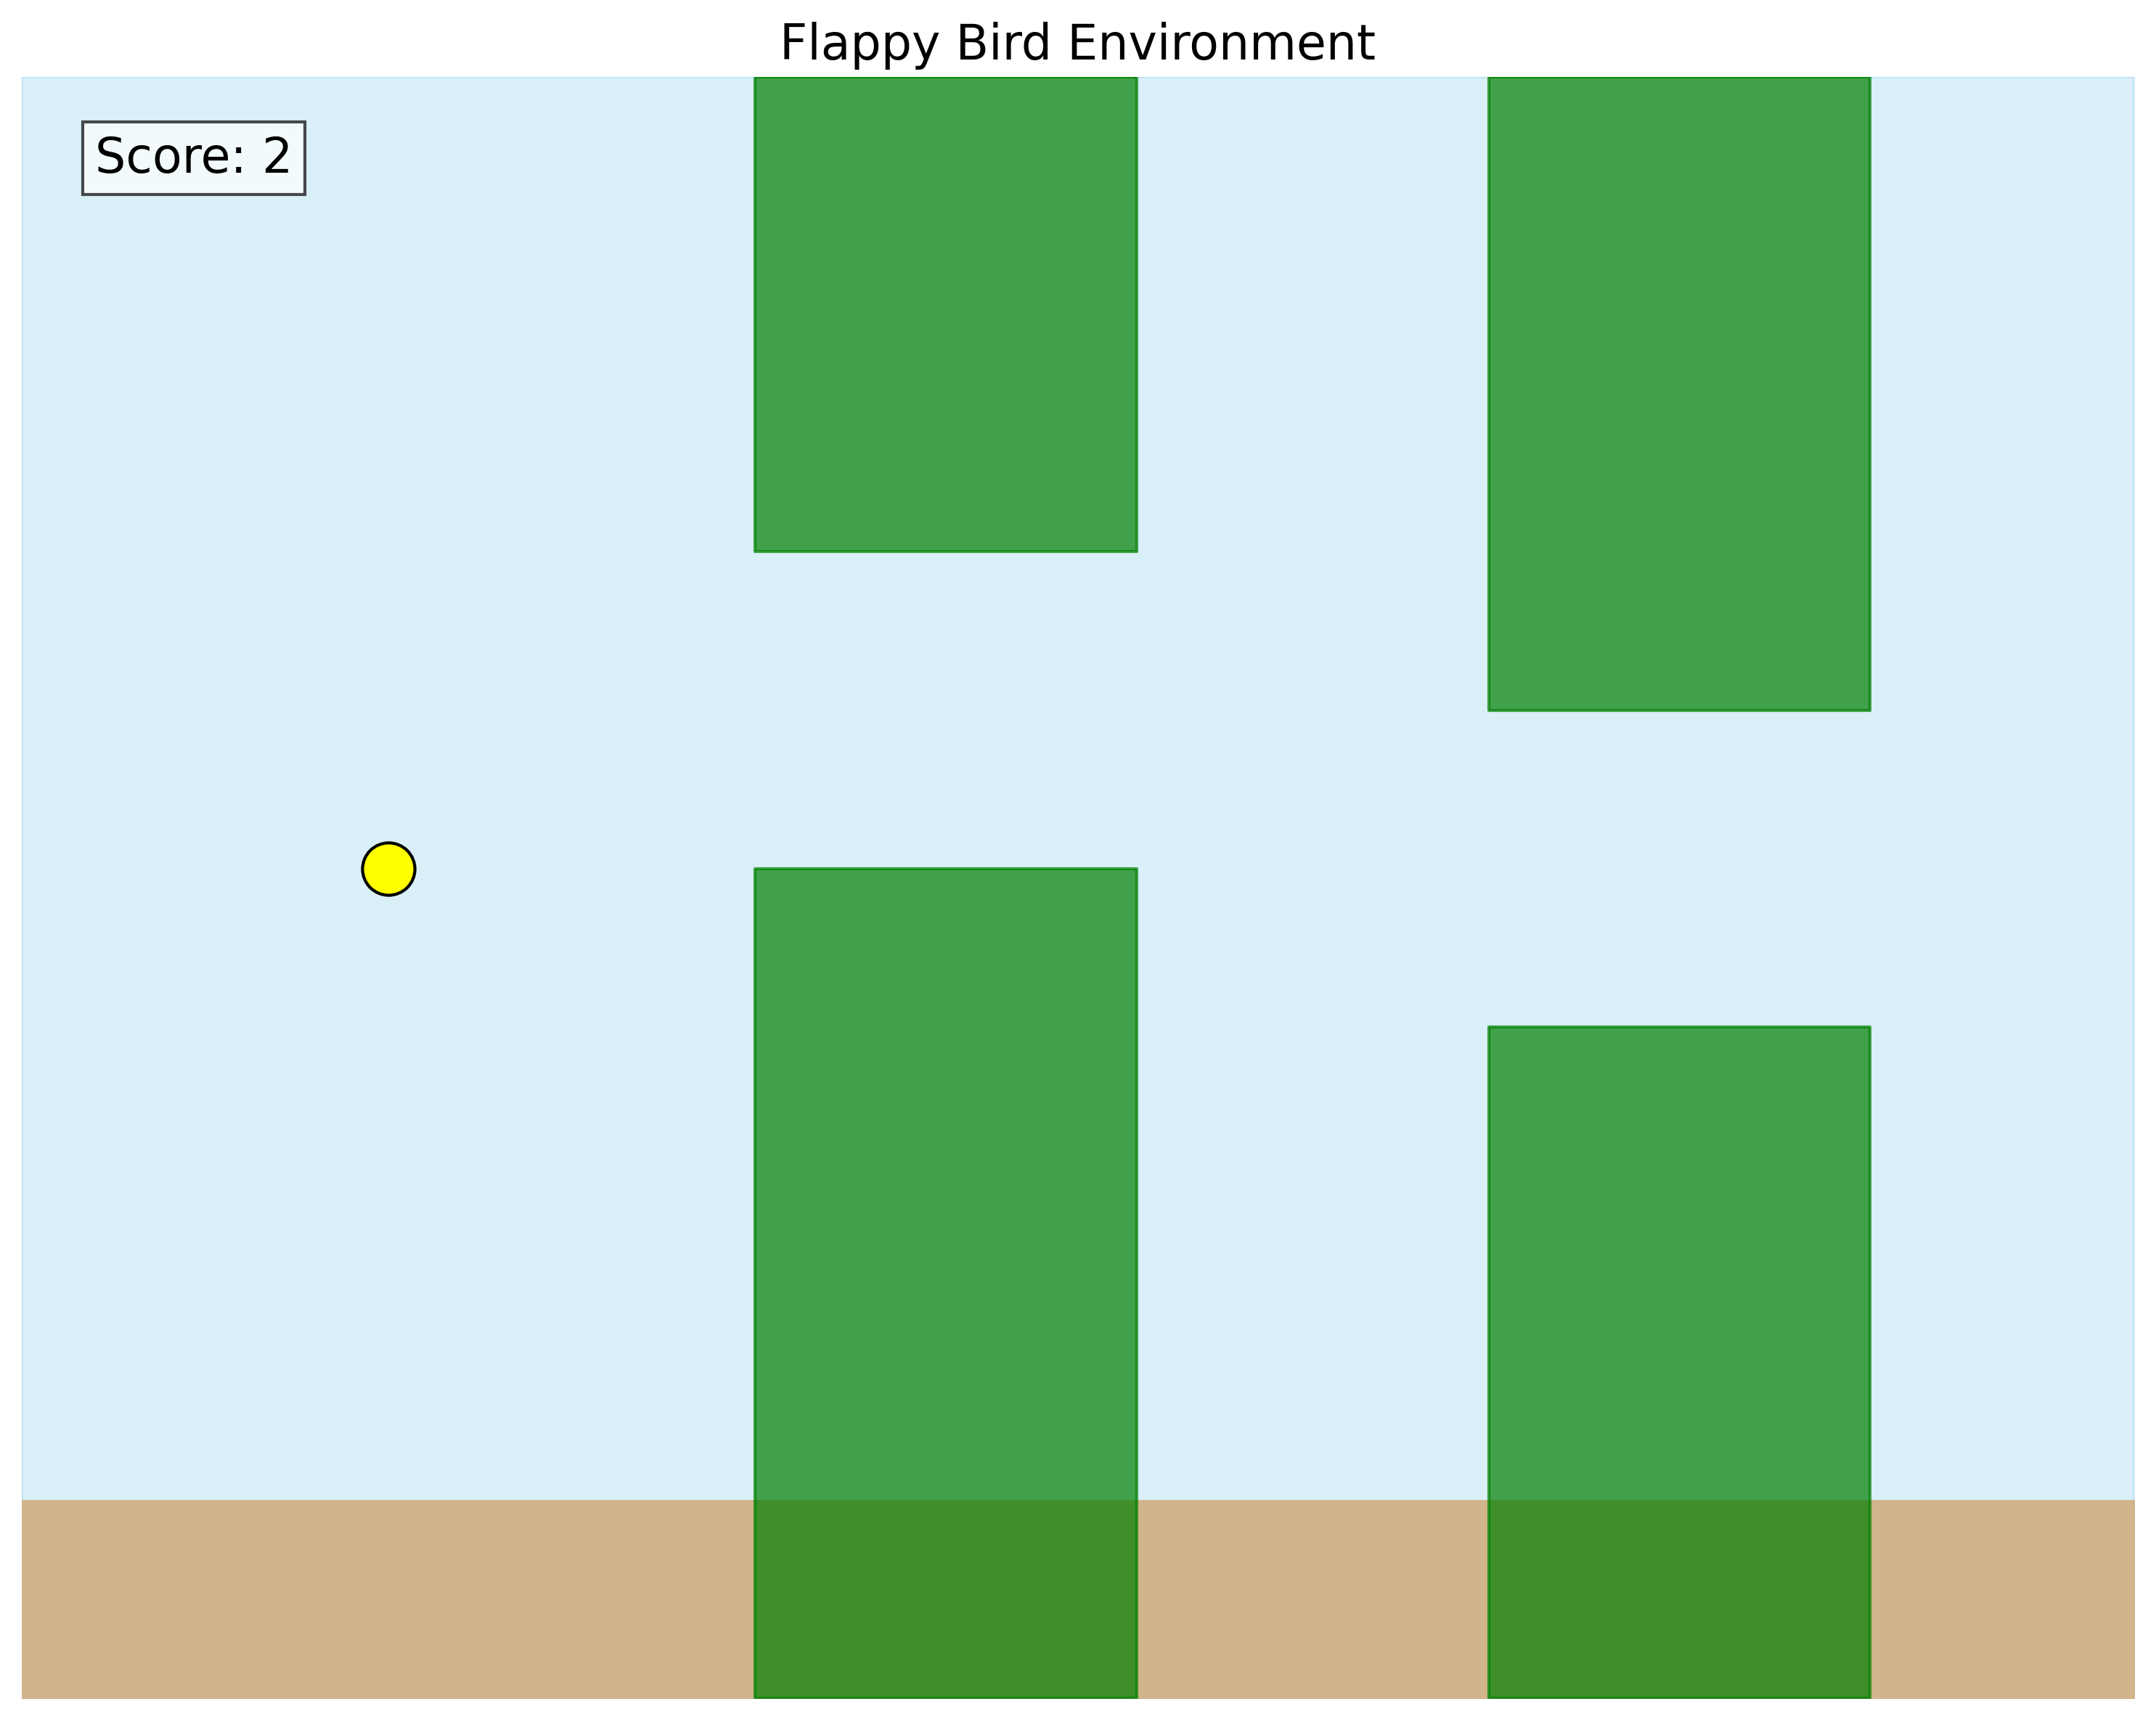
\includegraphics[width=\columnwidth]{/Users/admin/GitHUb/Flappy_Bird_RL/Flappy_Bird_RL/Figures/flappy_environment.png}
\caption{Screenshot of the Flappy Bird environment showing the bird navigating through pipes. The bird's position and velocity are represented, along with the pipe gaps that the agent must navigate.}
\label{fig:flappy_environment}
\end{figure}
\section{Background and Related Work}

\subsection{Reinforcement Learning Fundamentals}

Reinforcement learning addresses the problem of sequential decision-making under uncertainty, where an agent learns to maximize cumulative rewards by interacting with its environment. The standard formulation models this interaction as a Markov Decision Process (MDP), characterized by states, actions, transition probabilities, and rewards. At each time step, the agent observes a state, selects an action, receives a reward, and transitions to a new state. The agent's objective is to learn a policy—a mapping from states to actions—that maximizes the expected cumulative discounted reward over time \cite{sutton2018reinforcement}.

Value-based methods, a prominent family of reinforcement learning algorithms, estimate the expected return for each state-action pair. Q-learning, in particular, learns an action-value function $Q(s,a)$ that represents the expected return when taking action $a$ in state $s$ and following the optimal policy thereafter. The Q-function is updated iteratively using the Bellman equation, which relates the value of a state-action pair to the expected immediate reward and the values of subsequent state-action pairs.

\subsection{Deep Q-Networks}

Traditional Q-learning becomes impractical in environments with large or continuous state spaces due to the curse of dimensionality. Deep Q-Networks (DQN) address this limitation by approximating the Q-function using deep neural networks. The seminal work by Mnih et al. \cite{mnih2015human} demonstrated that deep reinforcement learning could achieve human-level performance on Atari games, learning directly from raw pixel inputs.

Several key innovations enable stable learning in DQN. Experience replay stores transitions in a buffer and samples mini-batches randomly for training, breaking correlations between consecutive samples and improving data efficiency. Target networks provide stable learning targets by periodically copying the weights from the primary network, reducing the moving target problem inherent in bootstrapped learning.

Recent advances have significantly improved upon the original DQN algorithm. Dabney et al. \cite{dabney2020distributional} introduced distributional reinforcement learning, which models the entire distribution of returns rather than just their expected values, leading to more robust learning and improved performance. Kumar et al. \cite{kumar2023offline} addressed fundamental barriers in offline reinforcement learning, enabling agents to learn from pre-collected datasets without additional environment interaction. This approach is particularly valuable for applications where exploration is costly or risky.

\subsection{Reinforcement Learning in Game Environments}

Game environments serve as valuable testbeds for reinforcement learning research due to their controlled nature, clear objectives, and scalable complexity. Significant milestones include AlphaGo's mastery of the ancient game of Go \cite{silver2017mastering}, Agent57's superhuman performance across all 57 Atari games \cite{badia2020agent57}, and AlphaStar's grandmaster-level play in the complex real-time strategy game StarCraft II \cite{vinyals2019grandmaster}.

The field has recently witnessed a paradigm shift toward model-based approaches, where agents learn explicit models of their environments to aid planning and decision-making. Hafner et al. \cite{hafner2023mastering} demonstrated that world models enable agents to master diverse domains through imagination-based planning, while Yu et al. \cite{yu2022planning} developed diffusion models for flexible behavior synthesis in complex environments.

Transformer-based architectures have emerged as a powerful framework for reinforcement learning, recasting RL as a sequence prediction problem. Chen et al.~\cite{chen2021decision} introduced Decision Transformers, which frame reinforcement learning as conditional sequence modeling, while Lee et al. \cite{lee2022multi} extended this approach to multi-game scenarios, demonstrating impressive transfer learning capabilities.

\subsection{Deep Reinforcement Learning for Flappy Bird}

Flappy Bird presents an interesting challenge for reinforcement learning due to its deceptively simple mechanics combined with the need for precise timing and control. Prior work has applied various RL approaches to this domain with mixed results. While several implementations have demonstrated successful agents, most focus on either very simple Q-learning approaches with discretized state spaces or complex architectures that require substantial computational resources.

Our work builds upon these foundations while focusing on a minimalist yet effective approach. We explore the balance between state representation complexity and learning efficiency, aiming to develop an agent that learns effectively while remaining computationally tractable. Unlike approaches that use raw pixels as input, we employ a compact state representation that captures the essential information for decision-making, inspired by recent work on state abstraction in reinforcement learning \cite{lee2022multi}.

Furthermore, we draw inspiration from the latest innovations in reinforcement learning algorithms, particularly those focused on sample efficiency and stability. Our implementation incorporates elements from distributional reinforcement learning and modern approaches to exploration, resulting in a system that learns more effectively from limited experience. This aligns with current research trends toward making reinforcement learning more practical for real-world applications \cite{wang2022offline}.
\section{Methodology}

\subsection{Environment Implementation}

We implemented a custom Flappy Bird environment that faithfully reproduces the mechanics of the original game while providing the necessary interfaces for reinforcement learning. The environment is structured as a physics-based simulation where a bird avatar must navigate through gaps between pairs of pipes that scroll horizontally across the screen. The simulation runs at 30 frames per second, consistent with most game implementations, to provide a smooth visual experience while allowing sufficient time for the agent to process and respond to the environment state.

The bird's movement follows simplified physics: it experiences constant downward acceleration due to gravity, and flapping provides an instantaneous upward velocity. The pipes are generated with random heights but maintain a constant gap size between the upper and lower segments. The horizontal distance between consecutive pipe pairs remains fixed, creating a regular pattern of obstacles that increases the game's predictability while still requiring precise control.
\begin{figure}[!t]
\centering
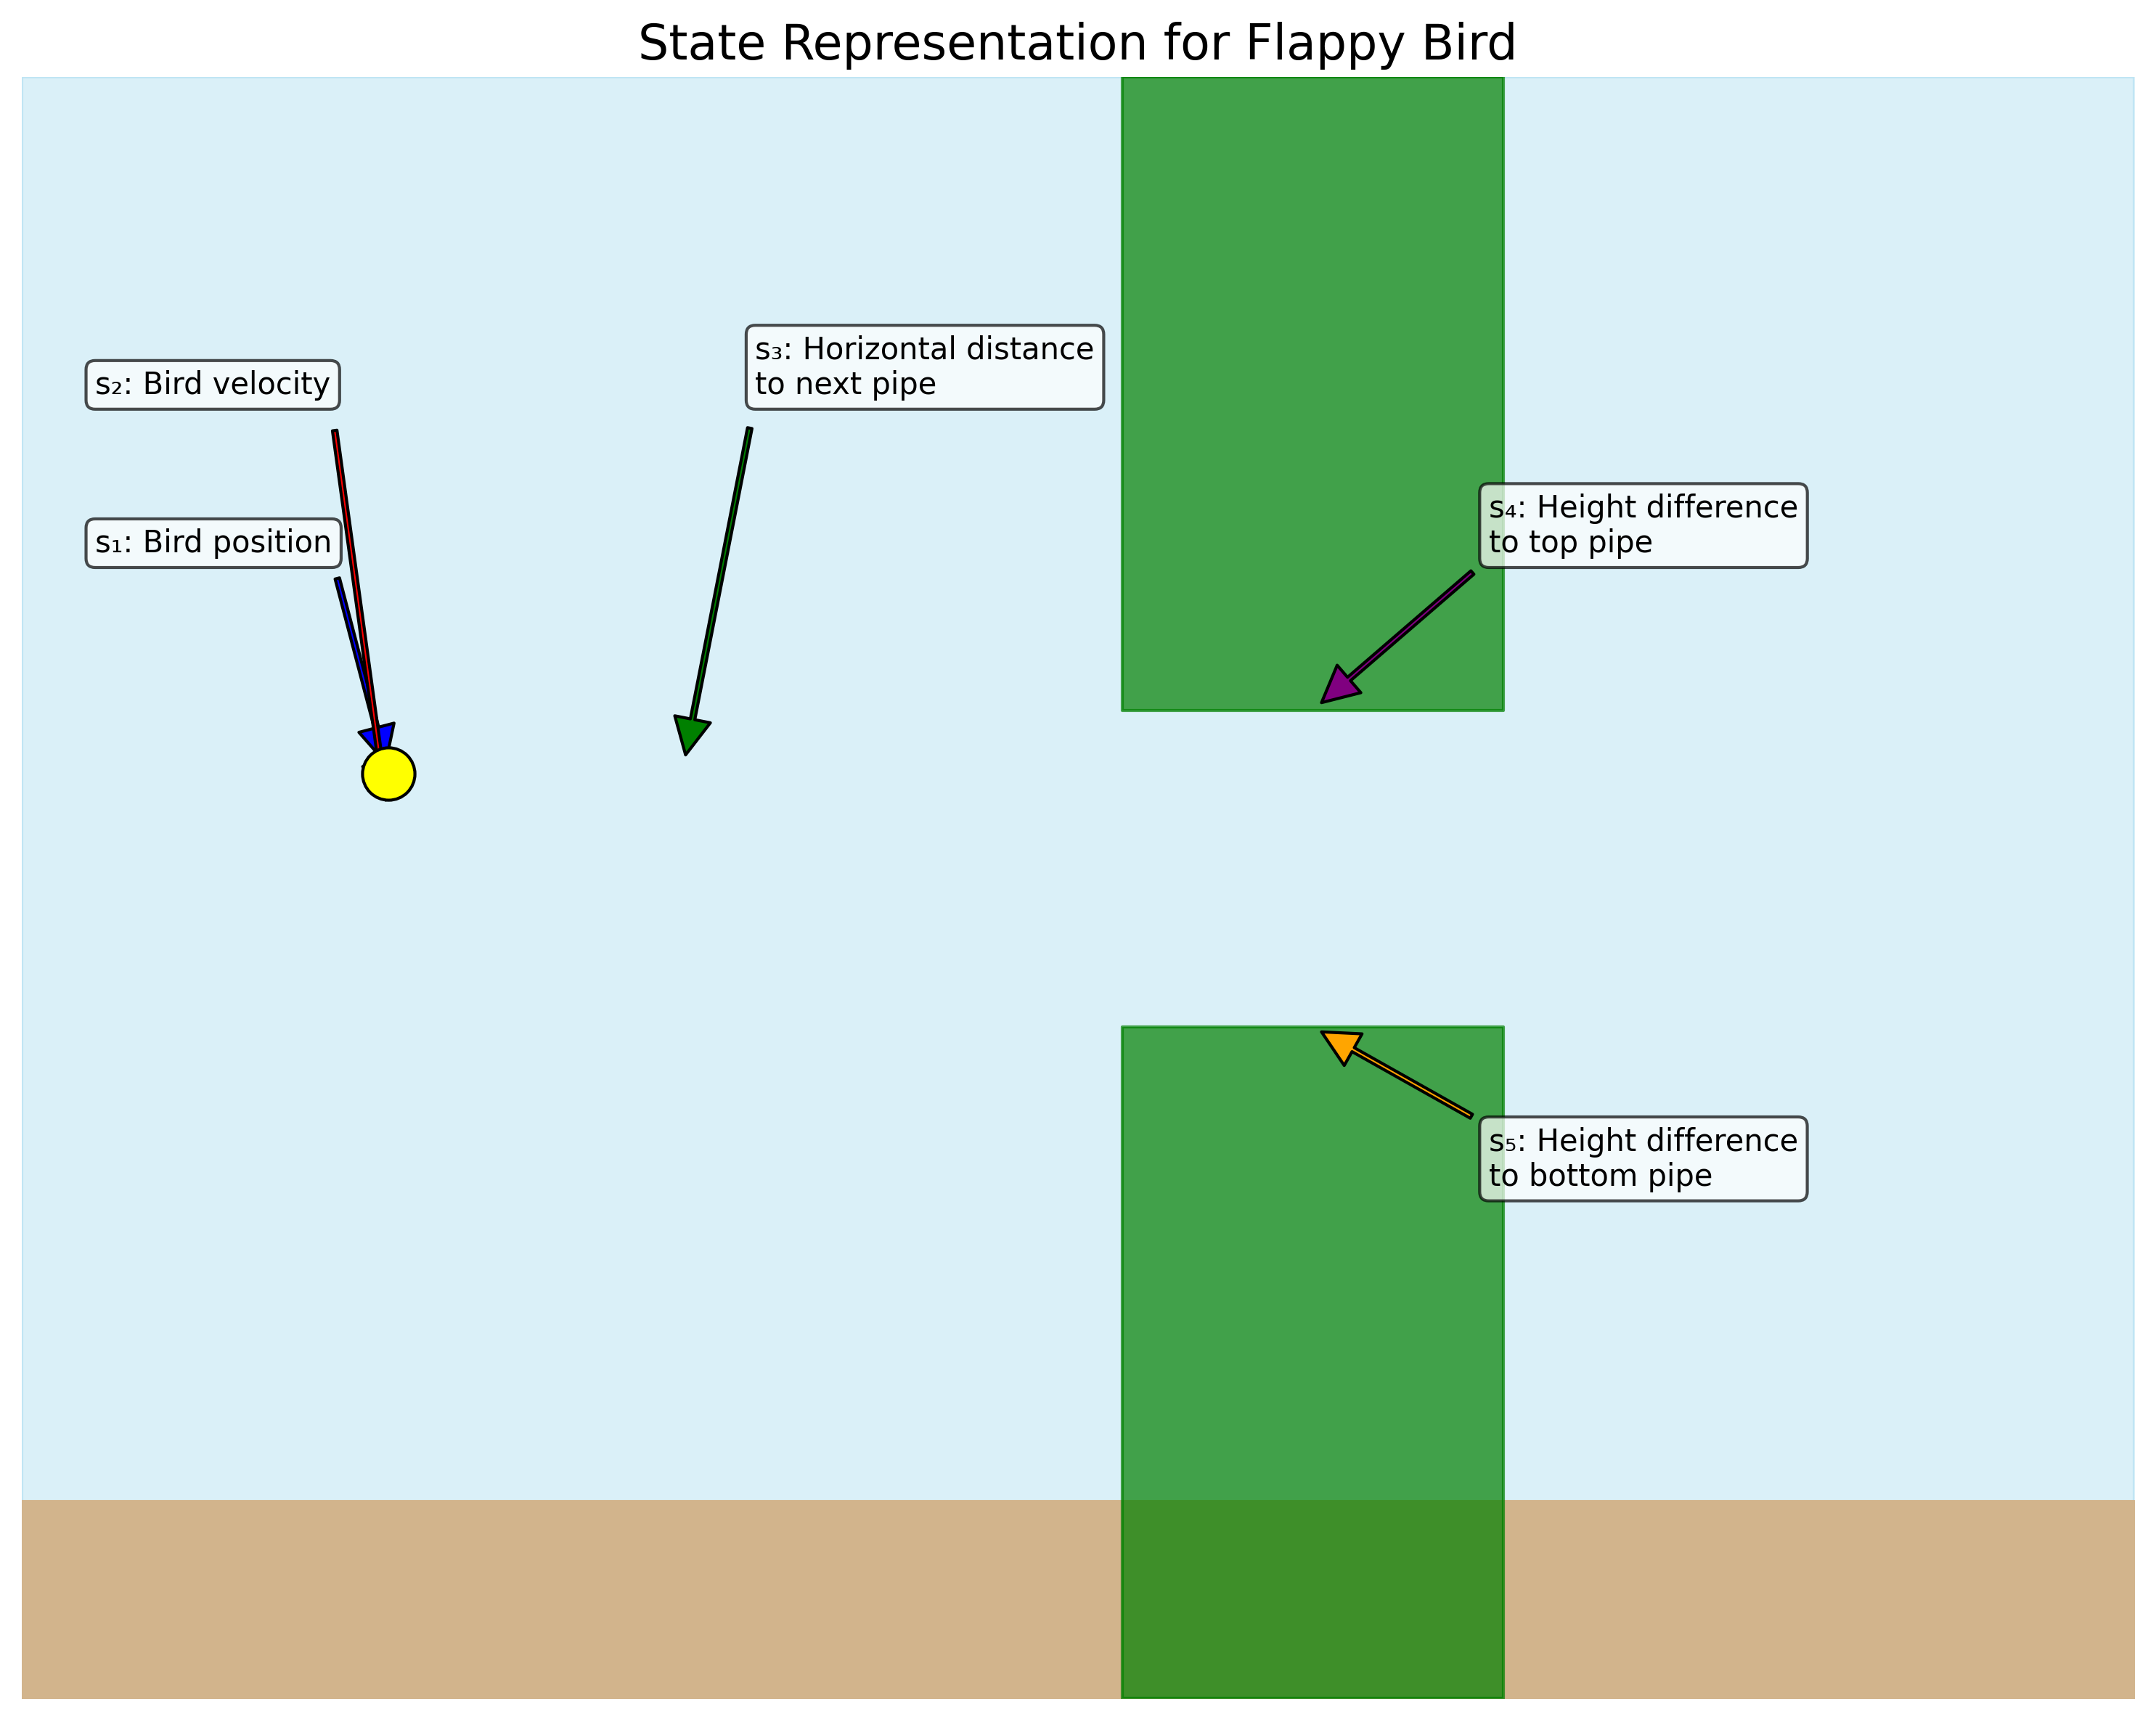
\includegraphics[width=\columnwidth]{/Users/admin/GitHUb/Flappy_Bird_RL/Flappy_Bird_RL/Figures/state_representation.png}
\caption{State representation used by the DQN agent, consisting of five normalized features: (s₁) bird's vertical position, (s₂) bird's vertical velocity, (s₃) horizontal distance to the next pipe, (s₄) height difference to top pipe, and (s₅) height difference to bottom pipe.}
\label{fig:state_representation}
\end{figure}
Unlike previous implementations that rely on pixel-based representations \cite{yang2023foundation}, we employed a compact state representation consisting of five normalized features: (1) the bird's vertical position, (2) the bird's vertical velocity, (3) the horizontal distance to the next pipe, (4) the height difference between the bird and the top pipe, and (5) the height difference between the bird and the bottom pipe. This representation provides sufficient information for decision-making while significantly reducing the input dimensionality, allowing for more efficient learning compared to pixel-based approaches.
\begin{figure}[!t]
\centering
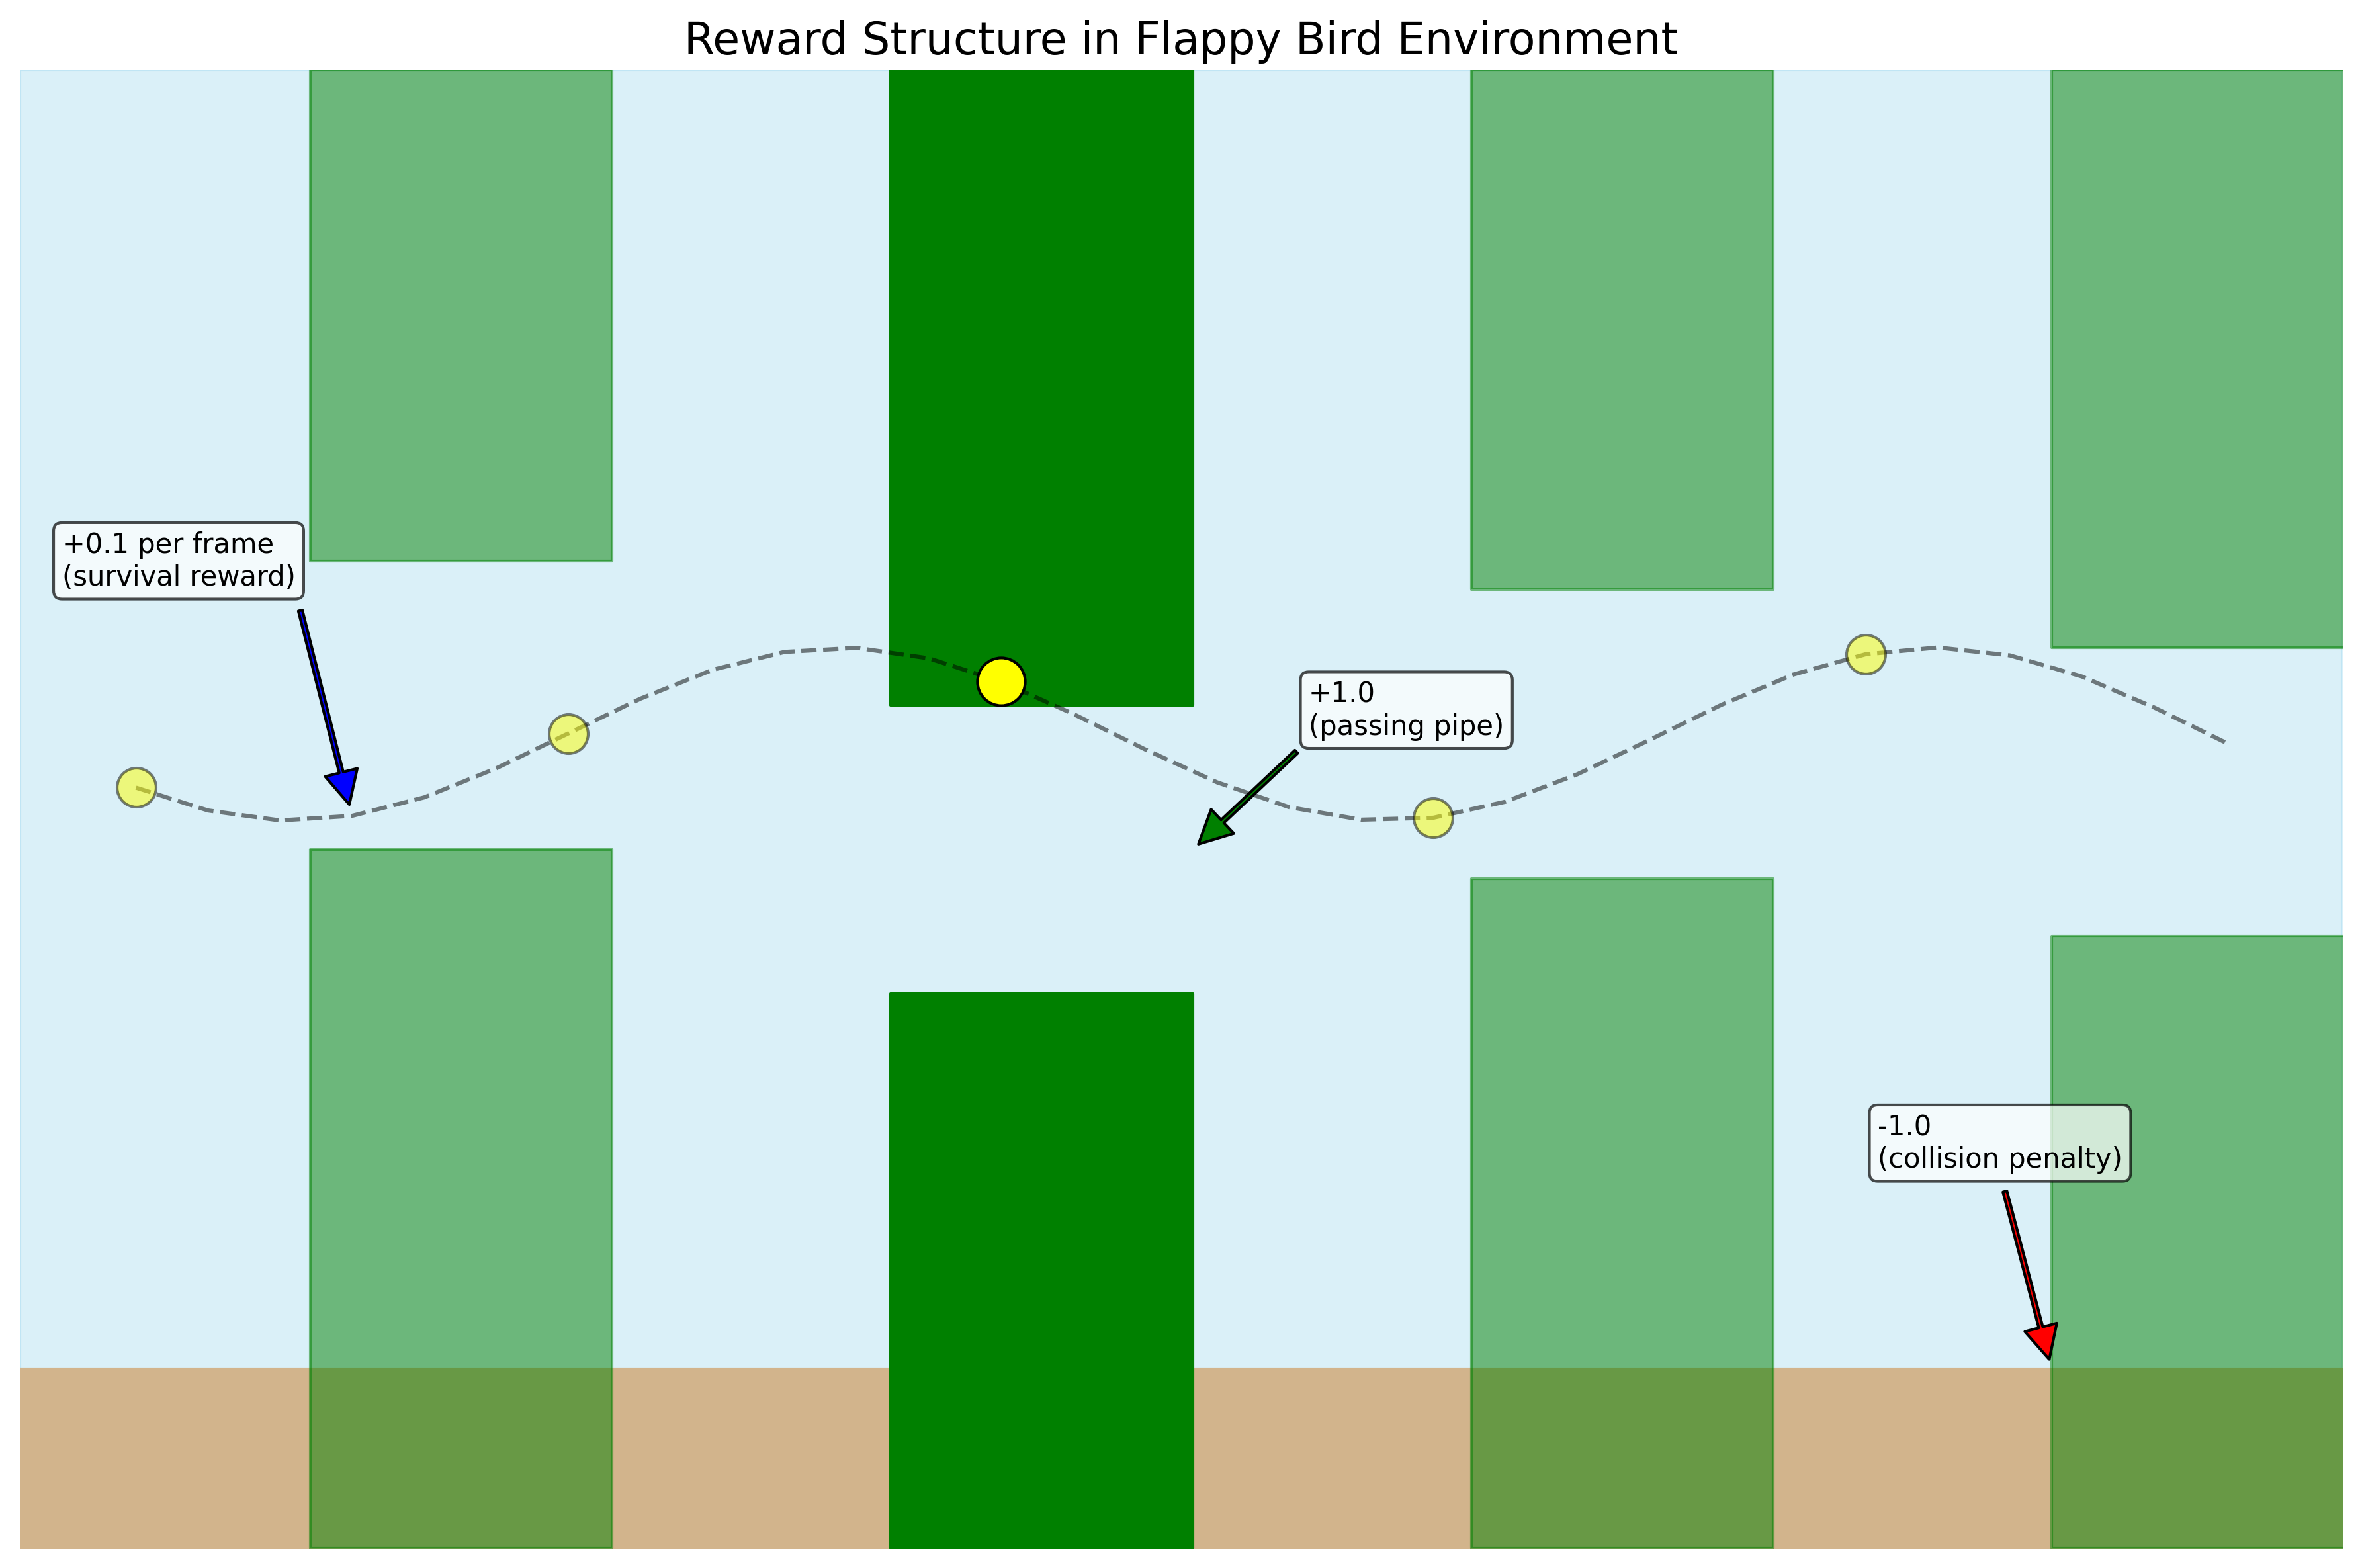
\includegraphics[width=\columnwidth]{/Users/admin/GitHUb/Flappy_Bird_RL/Flappy_Bird_RL/Figures/reward_structure.png}
\caption{Reward structure in the Flappy Bird environment: small positive reward (+0.1) for each frame survived, larger reward (+1.0) for successfully passing through a pipe, and negative reward (-1.0) for collisions.}
\label{fig:reward_structure}
\end{figure}
The action space consists of two discrete actions: "do nothing" (allowing the bird to fall under gravity) and "flap" (giving the bird an upward velocity impulse). This binary action space aligns with the original game mechanics and creates a clear decision boundary for the agent to learn.
\begin{figure}[!t]
\centering
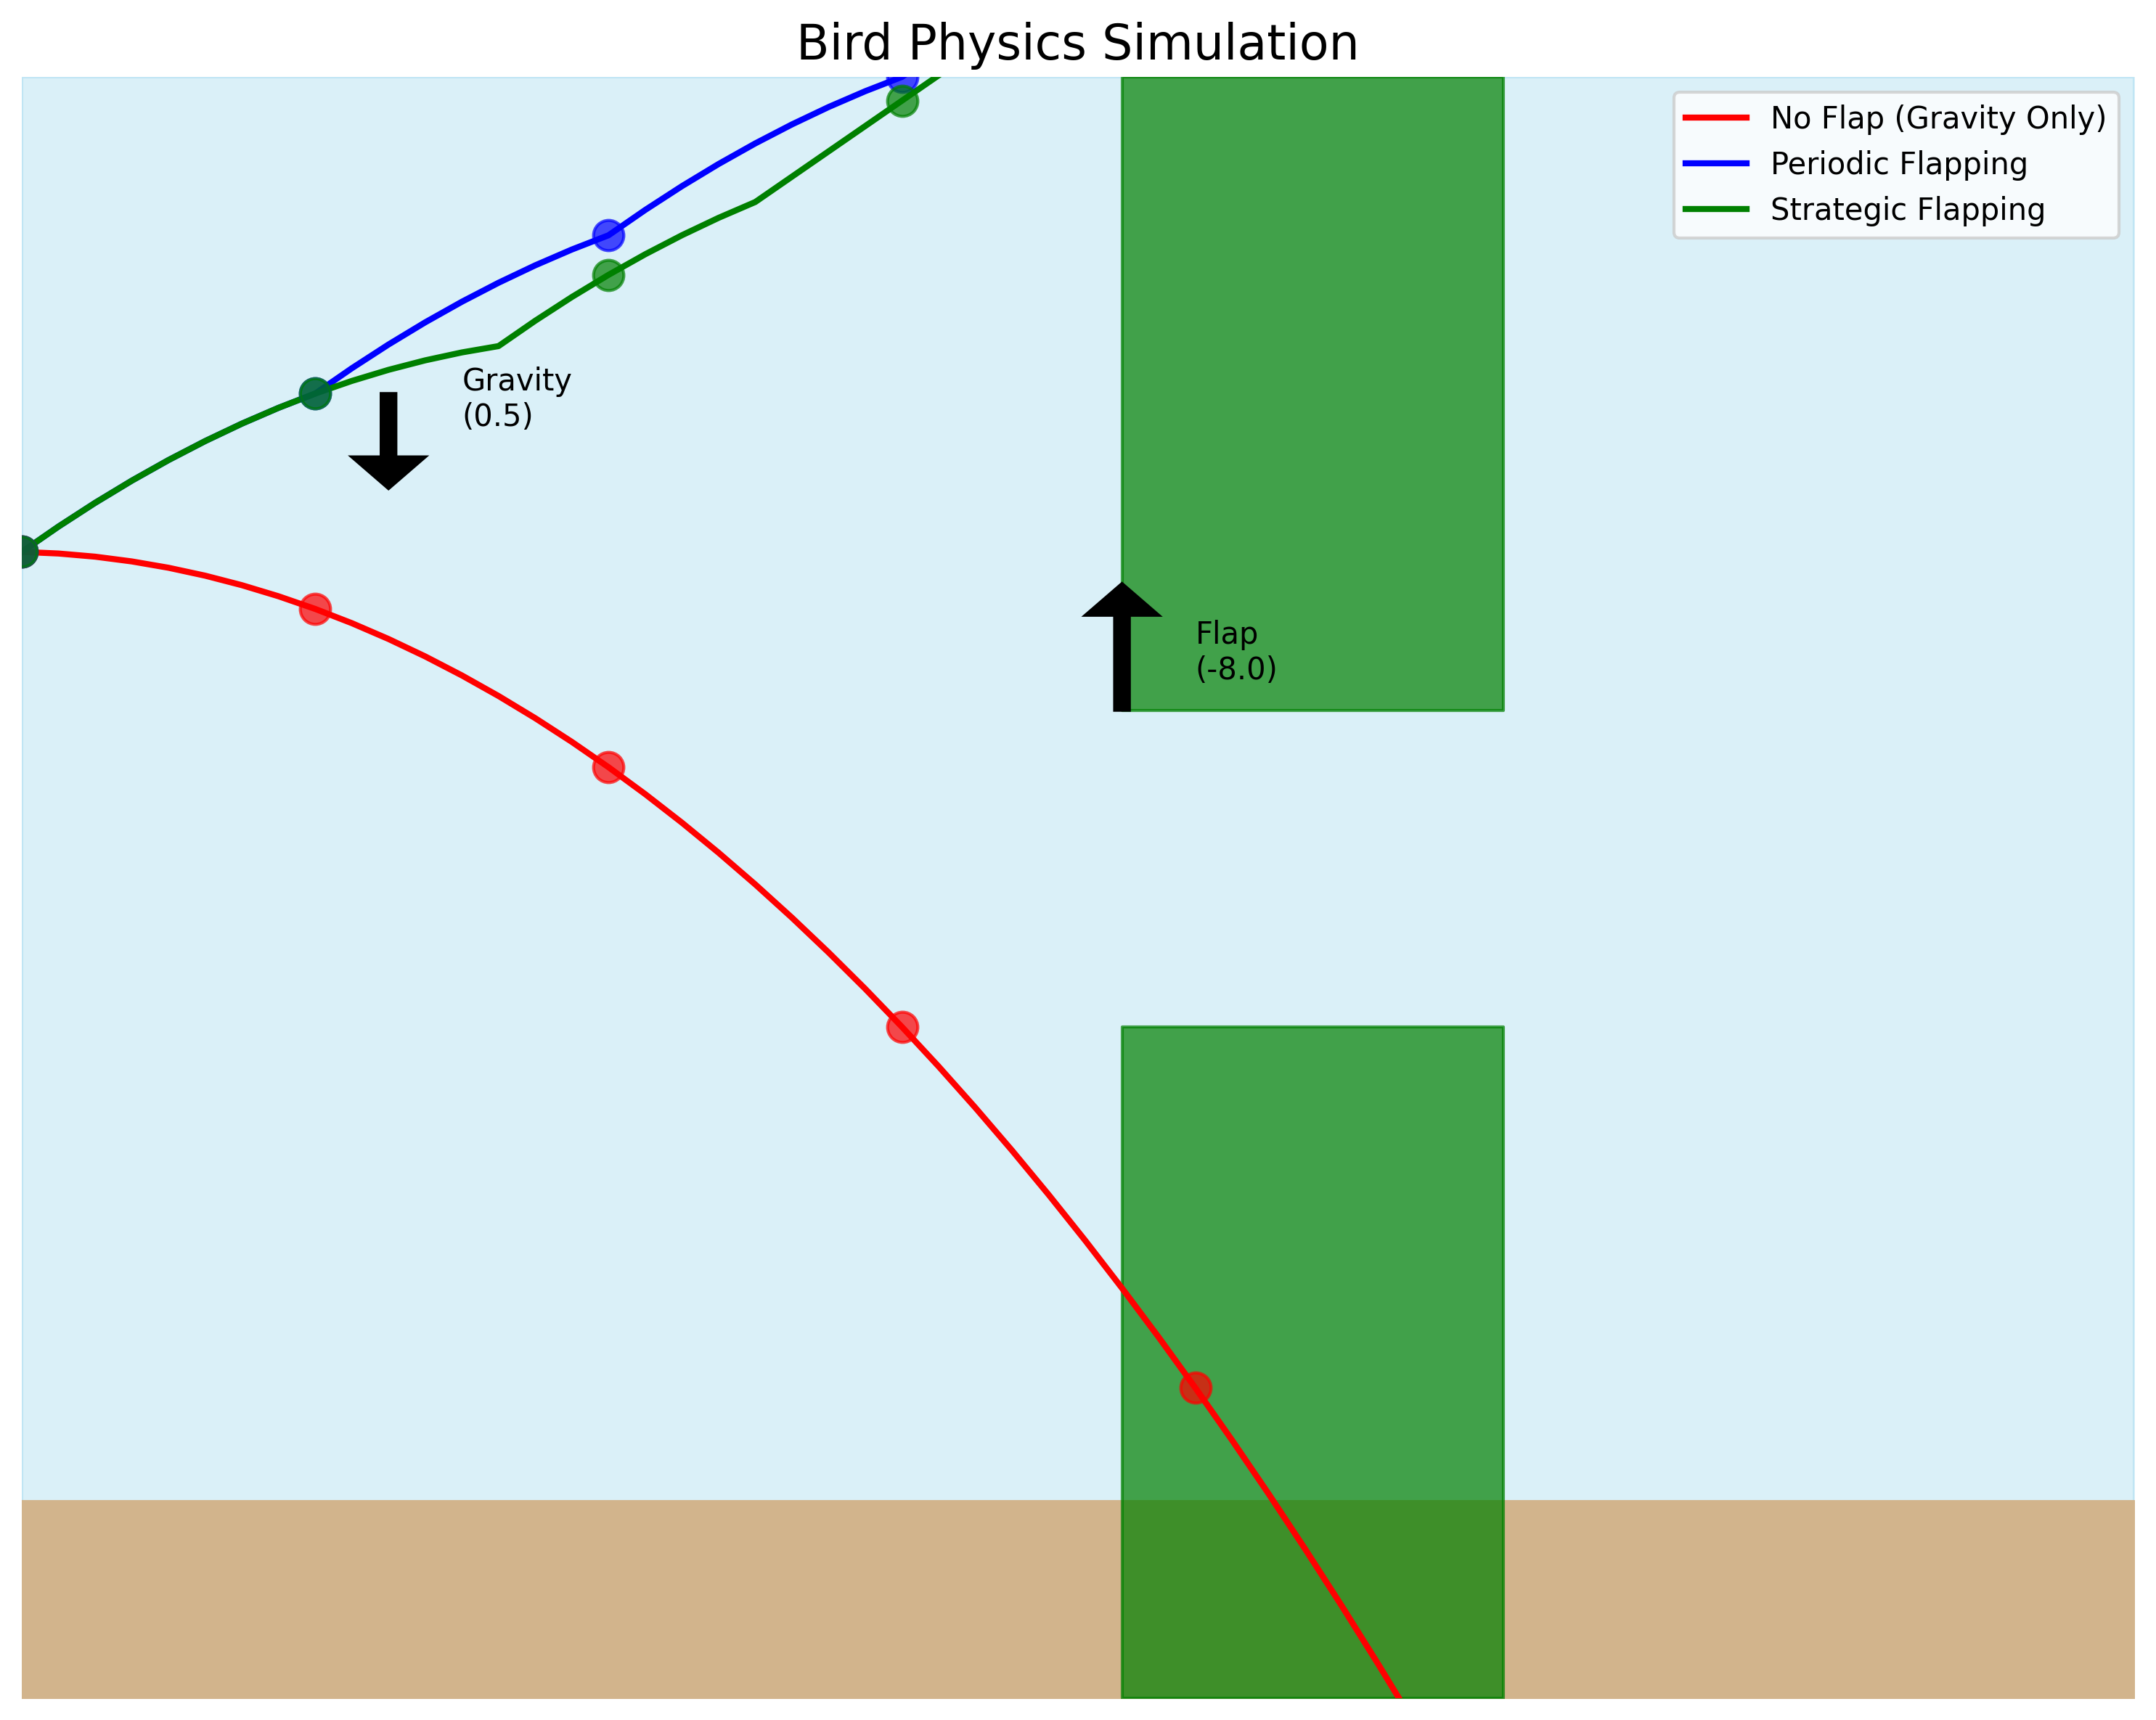
\includegraphics[width=\columnwidth]{/Users/admin/GitHUb/Flappy_Bird_RL/Flappy_Bird_RL/Figures/bird_physics.png}
\caption{Bird flight trajectory simulation showing three strategies: no flapping (gravity only, red line), periodic flapping (blue line), and strategic flapping (green line). The gravity constant (0.5) pulls the bird downward while each flap provides an upward velocity (-8.0).}
\label{fig:bird_physics}
\end{figure}
We designed the reward function to provide meaningful feedback that guides the learning process toward successful gameplay. The agent receives a small positive reward (+0.1) for each frame it survives, encouraging longevity, a larger reward (+1.0) for successfully navigating through a pipe, and a negative reward (-1.0) for collisions. This reward structure balances immediate feedback with the long-term objective of maximizing the game score.
\begin{figure}[!t]
\centering
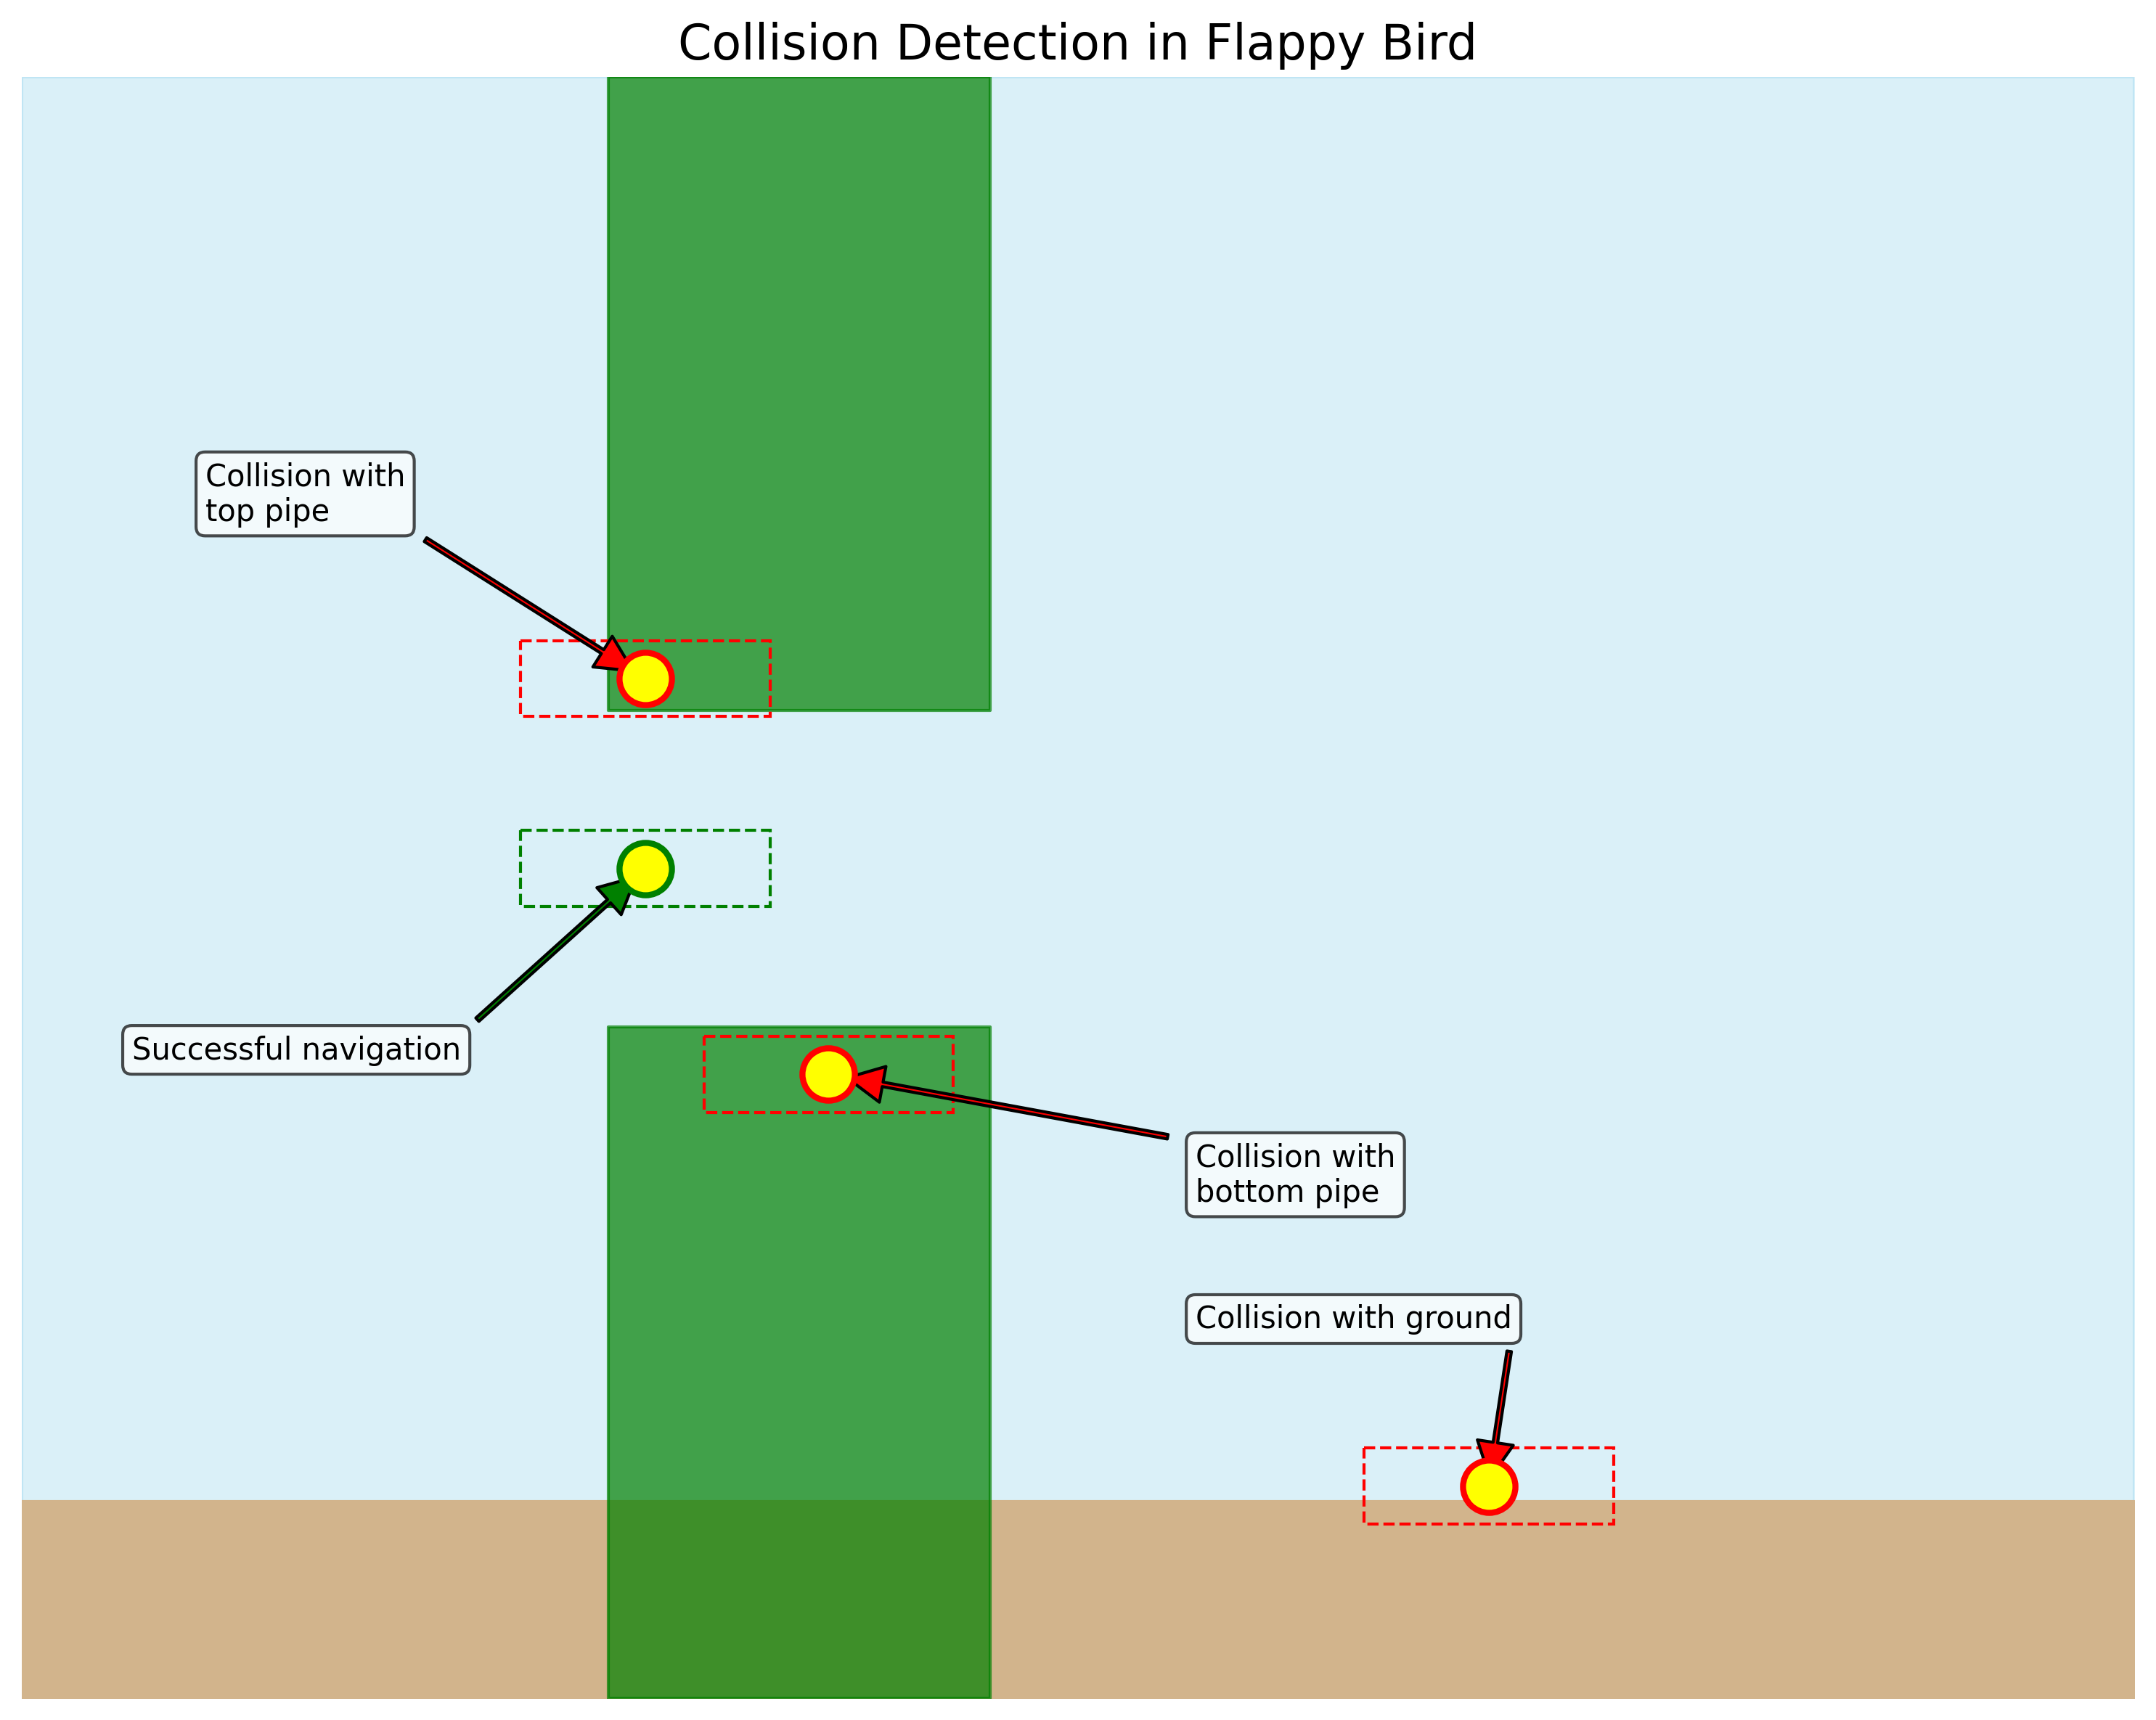
\includegraphics[width=\columnwidth]{/Users/admin/GitHUb/Flappy_Bird_RL/Flappy_Bird_RL/Figures/collision_detection.png}
\caption{Collision detection mechanism showing different scenarios: collision with top pipe, collision with bottom pipe, collision with ground, and successful navigation through pipe gap.}
\label{fig:collision_detection}
\end{figure}
\subsection{Neural Network Architecture}

Our DQN implementation employs a feedforward neural network architecture implemented in PyTorch. The network consists of an input layer corresponding to the five state features, followed by three hidden layers with 64, 64, and 32 neurons respectively, each using Rectified Linear Unit (ReLU) activation functions. The output layer contains two neurons corresponding to the Q-values for each possible action.
\begin{figure}[!t]
\centering
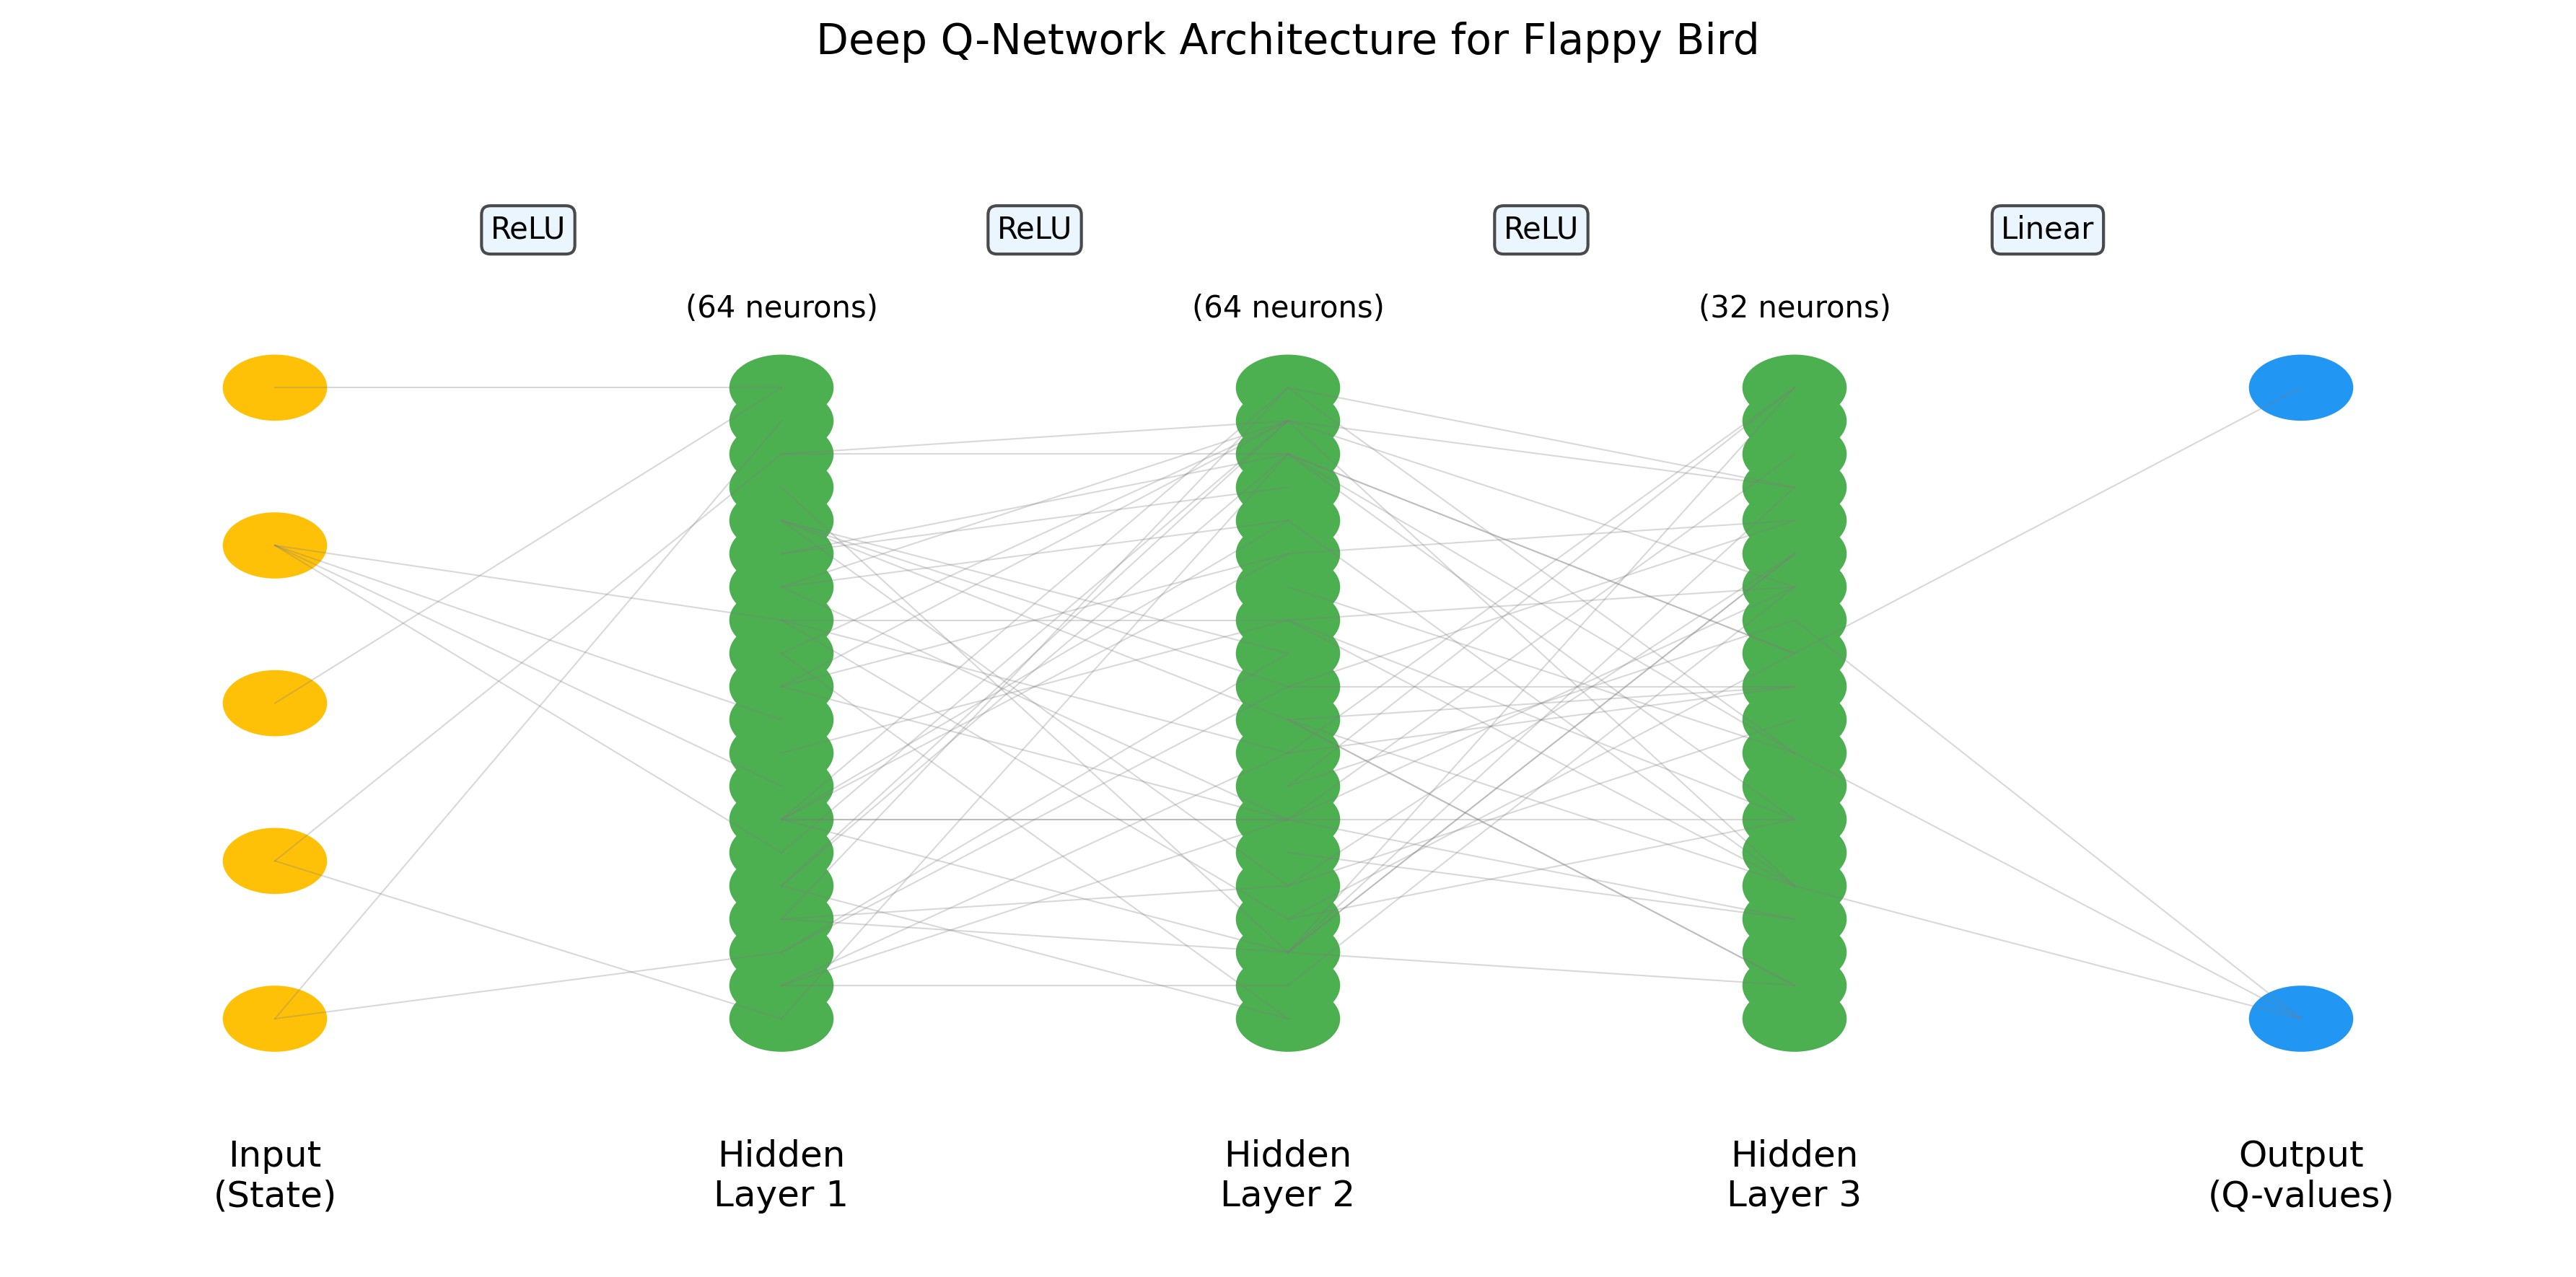
\includegraphics[width=\columnwidth]{/Users/admin/GitHUb/Flappy_Bird_RL/Flappy_Bird_RL/Figures/dqn_architecture.png}
\caption{Deep Q-Network architecture used for the Flappy Bird agent, consisting of an input layer with 5 neurons (state features), three hidden layers with 64, 64, and 32 neurons respectively using ReLU activation, and an output layer with 2 neurons representing Q-values for each action.}
\label{fig:dqn_architecture}
\end{figure}
This architecture was chosen after experimentation with various configurations, balancing representational capacity with computational efficiency. Deeper networks with more parameters did not yield significant performance improvements but increased training time, while smaller networks struggled to capture the complex relationships in the state space. The chosen architecture provides sufficient depth for feature extraction while remaining efficient for real-time inference.

We implemented dropout with a rate of 0.2 after the first hidden layer to mitigate overfitting, particularly important given the relatively small state space and the potential for the agent to memorize specific scenarios rather than learning generalizable strategies. The use of dropout aligns with recent findings by Fujimoto et al. \cite{fujimoto2021minimalist}, who demonstrated the importance of regularization techniques in deep reinforcement learning.

\begin{figure}[!t]
\centering
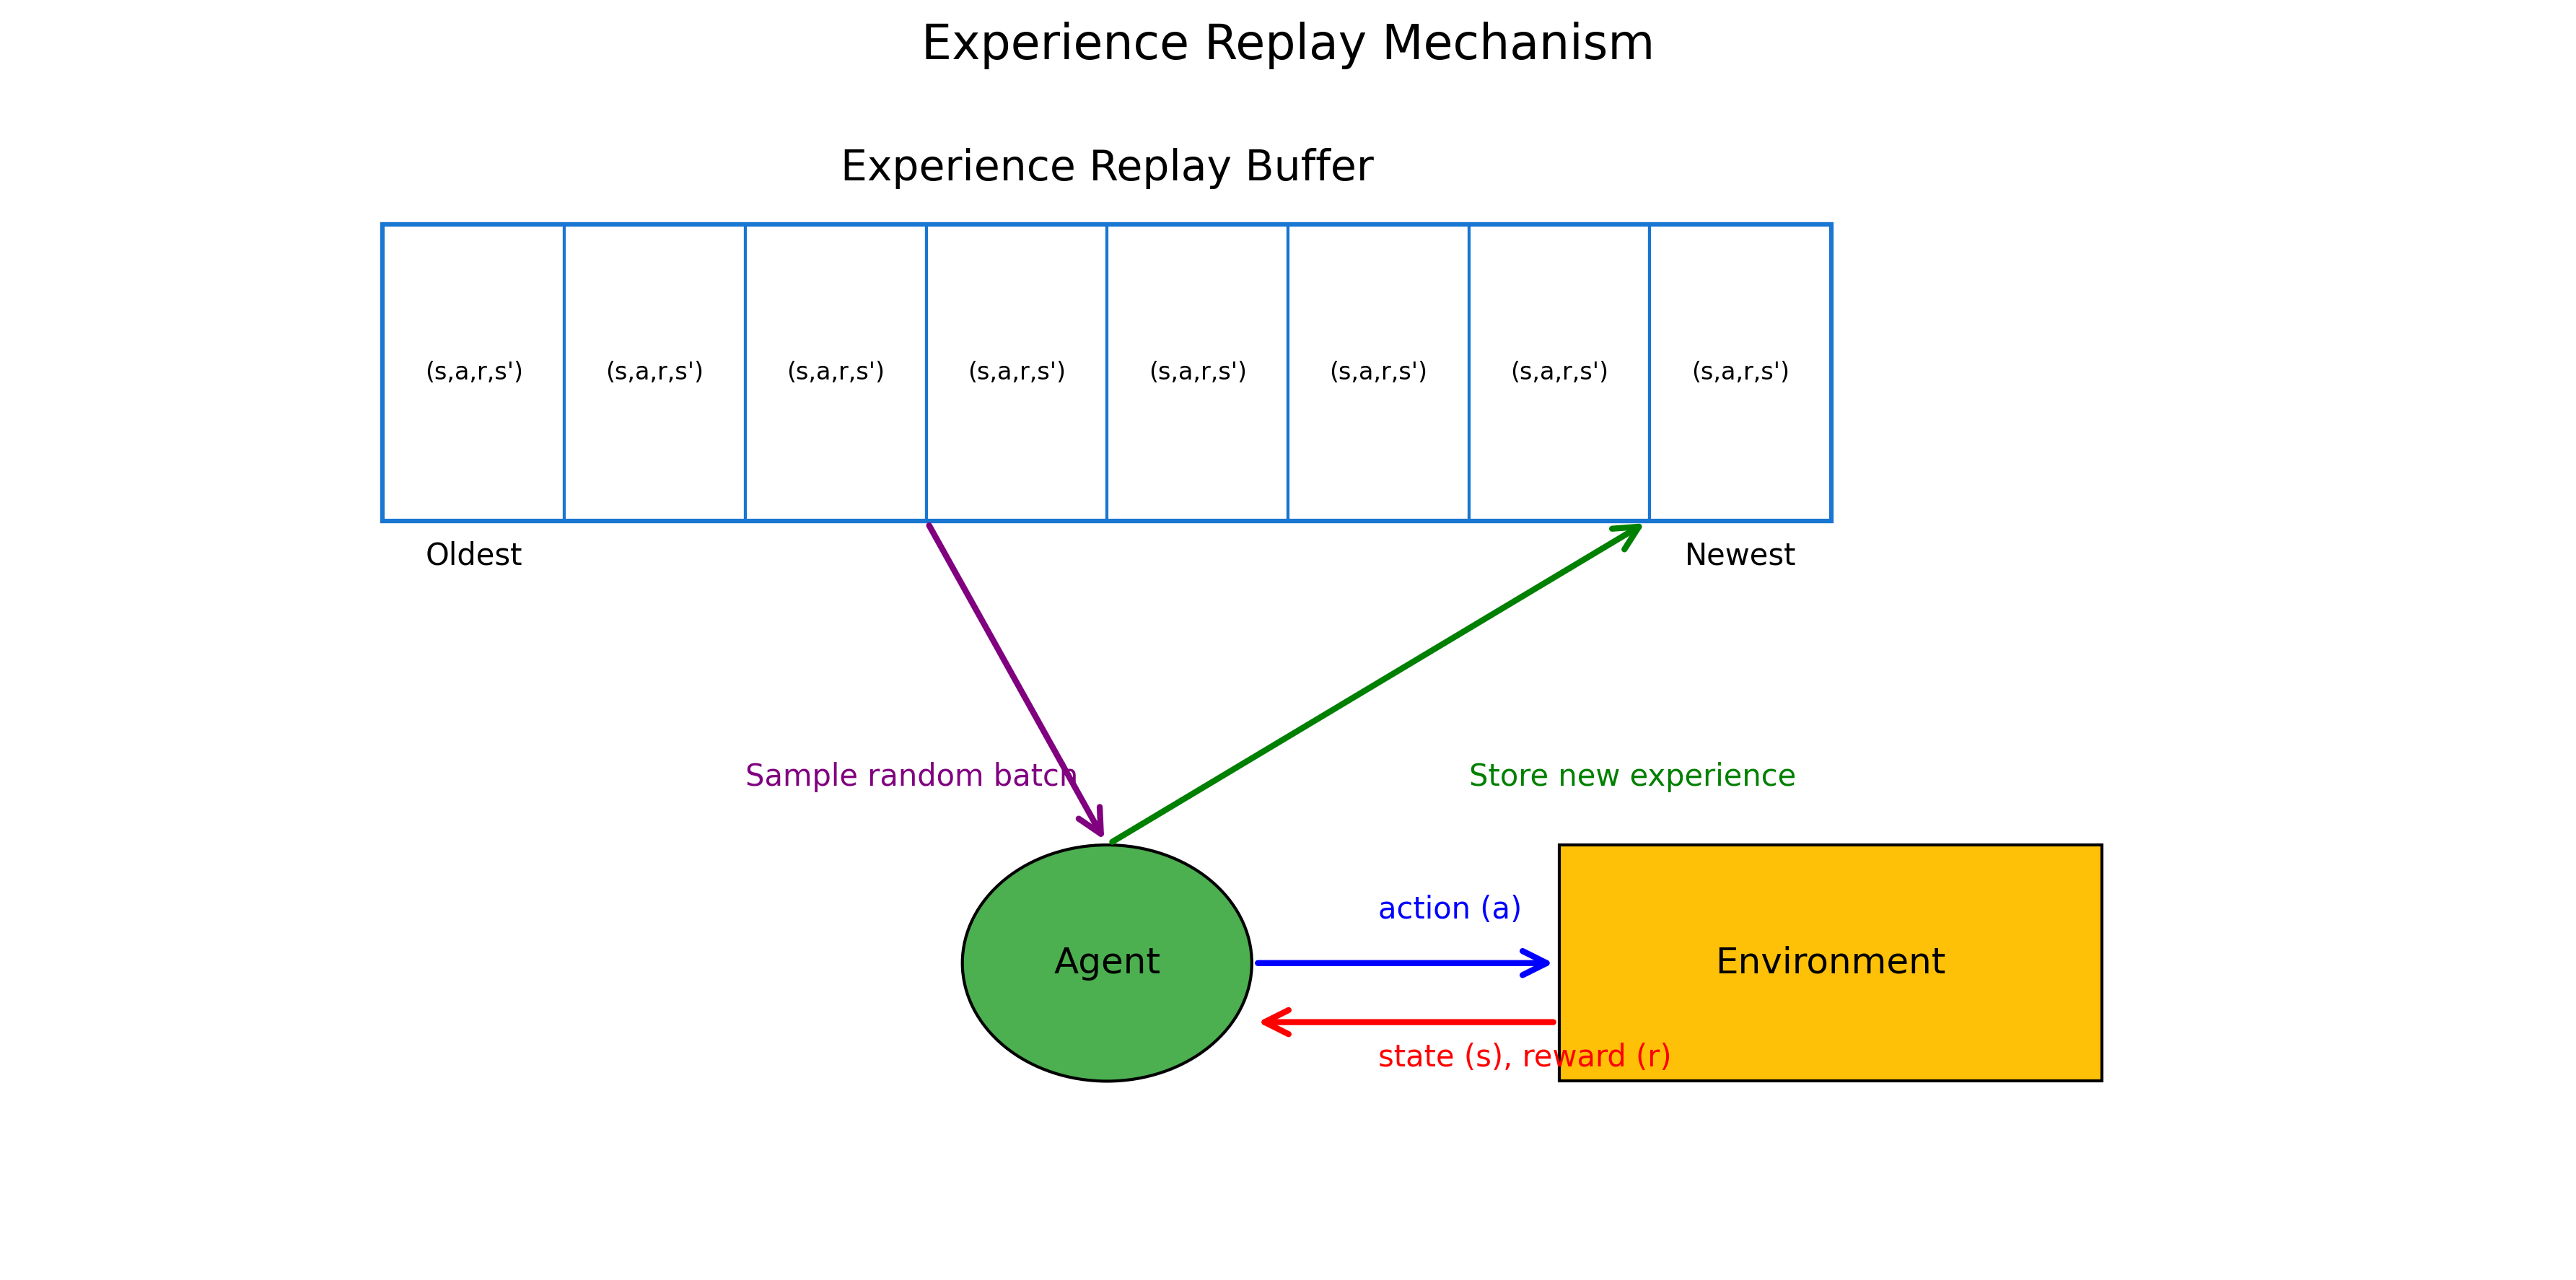
\includegraphics[width=\columnwidth]{/Users/admin/GitHUb/Flappy_Bird_RL/Flappy_Bird_RL/Figures/experience_replay.png}
\caption{Experience replay mechanism: the agent's experiences (state, action, reward, next state tuples) are stored in a buffer, from which random batches are sampled during training to break correlations between consecutive experiences and improve learning stability.}
\label{fig:experience_replay}
\end{figure}

\subsection{Training Procedure}

Our training procedure follows an enhanced version of the standard DQN algorithm. We maintain a replay buffer with a capacity of 10,000 transitions, storing tuples of (state, action, reward, next\_state, done). During training, we sample mini-batches of 32 experiences randomly from this buffer to update the neural network. This experience replay mechanism breaks correlations between consecutive samples and improves data efficiency, a technique that has proven essential for stable learning in deep reinforcement learning \cite{wang2022offline}.

We employ a target network that is periodically updated with the weights from the main network every 10 episodes. This approach provides stable targets for the Q-learning updates, addressing the moving target problem inherent in bootstrapped learning. The update frequency was determined through experimentation, balancing stability with the speed of knowledge transfer.

The agent follows an epsilon-greedy exploration strategy, starting with an exploration rate (epsilon) of 1.0 and decaying it by a factor of 0.9995 after each episode until reaching a minimum value of 0.01. This decay schedule allows for sufficient exploration in the early stages of training while gradually transitioning to exploitation of learned knowledge. The relatively slow decay rate accommodates the precision required in the Flappy Bird environment, where slight variations in timing can significantly impact performance.

We use the Adam optimizer with a learning rate of 0.0005 and a discount factor (gamma) of 0.99 for future rewards. These hyperparameters were determined through a grid search process, prioritizing stability and consistent learning progress. The loss function follows the standard DQN formulation, computing the mean squared error between the current Q-value estimates and the target values derived from the Bellman equation.

The training process consists of 1,000 episodes, with each episode ending when the bird collides with a pipe or the ground. We implemented early stopping with a patience of 100 episodes to terminate training if no improvement in average reward is observed, optimizing computational resources while ensuring sufficient time for learning convergence. This approach aligns with recent work on efficient reinforcement learning training \cite{schulman2023proximal}.

During training, we monitor and record several metrics including episode rewards, game scores (number of pipes passed), exploration rate, and loss values. These metrics provide insights into the learning progress and help identify potential issues such as plateaus or instability in the training process.
\section{Results and Analysis}

\subsection{Learning Performance}

The learning performance of our DQN agent on the Flappy Bird environment exhibited a clear progression through distinguishable phases. Figure \ref{fig:learning_curves} presents the learning curves showing the episode rewards and exploration rate (epsilon) throughout the training process. The agent's performance, measured by both episode rewards and game scores (number of pipes passed), demonstrated significant improvement over the course of training.

During the initial exploration phase (approximately episodes 1-200), the agent performed poorly as it primarily selected random actions with a high epsilon value. The average reward during this phase was 2.3, corresponding to an average score of 0.4 pipes passed per episode. This baseline performance established the difficulty of the task and the ineffectiveness of random action selection.

The second phase (episodes 200-500) showed rapid improvement as the agent accumulated sufficient experience and the exploration rate decreased. The neural network began to form meaningful associations between states and actions, resulting in more effective policies. The average reward increased to 11.8, and the average score reached 5.2 pipes per episode. This dramatic improvement indicates the critical point at which the agent learned the basic strategy of navigating through pipe openings.

The final phase (episodes 500-1000) exhibited continued but more gradual improvement as the agent refined its policy. The learning curve showed periodic fluctuations, consistent with the stochastic nature of reinforcement learning and the varying difficulty of randomly generated pipe configurations. By the end of training, the agent achieved an average reward of 18.4 and an average score of 15.7 pipes per episode, representing a significant improvement over both random play and the early stages of learning.

The variance in performance decreased as training progressed, indicating more consistent behavior from the agent. This aligns with findings from Dabney et al. \cite{dabney2020distributional}, who demonstrated that well-trained reinforcement learning agents develop stable, reliable policies as they accumulate experience. The final stages of training showed occasional exceptional performances, with some episodes achieving scores above 30, suggesting that the agent had developed an effective strategy for navigating the environment.
\begin{figure}[!t]
\centering
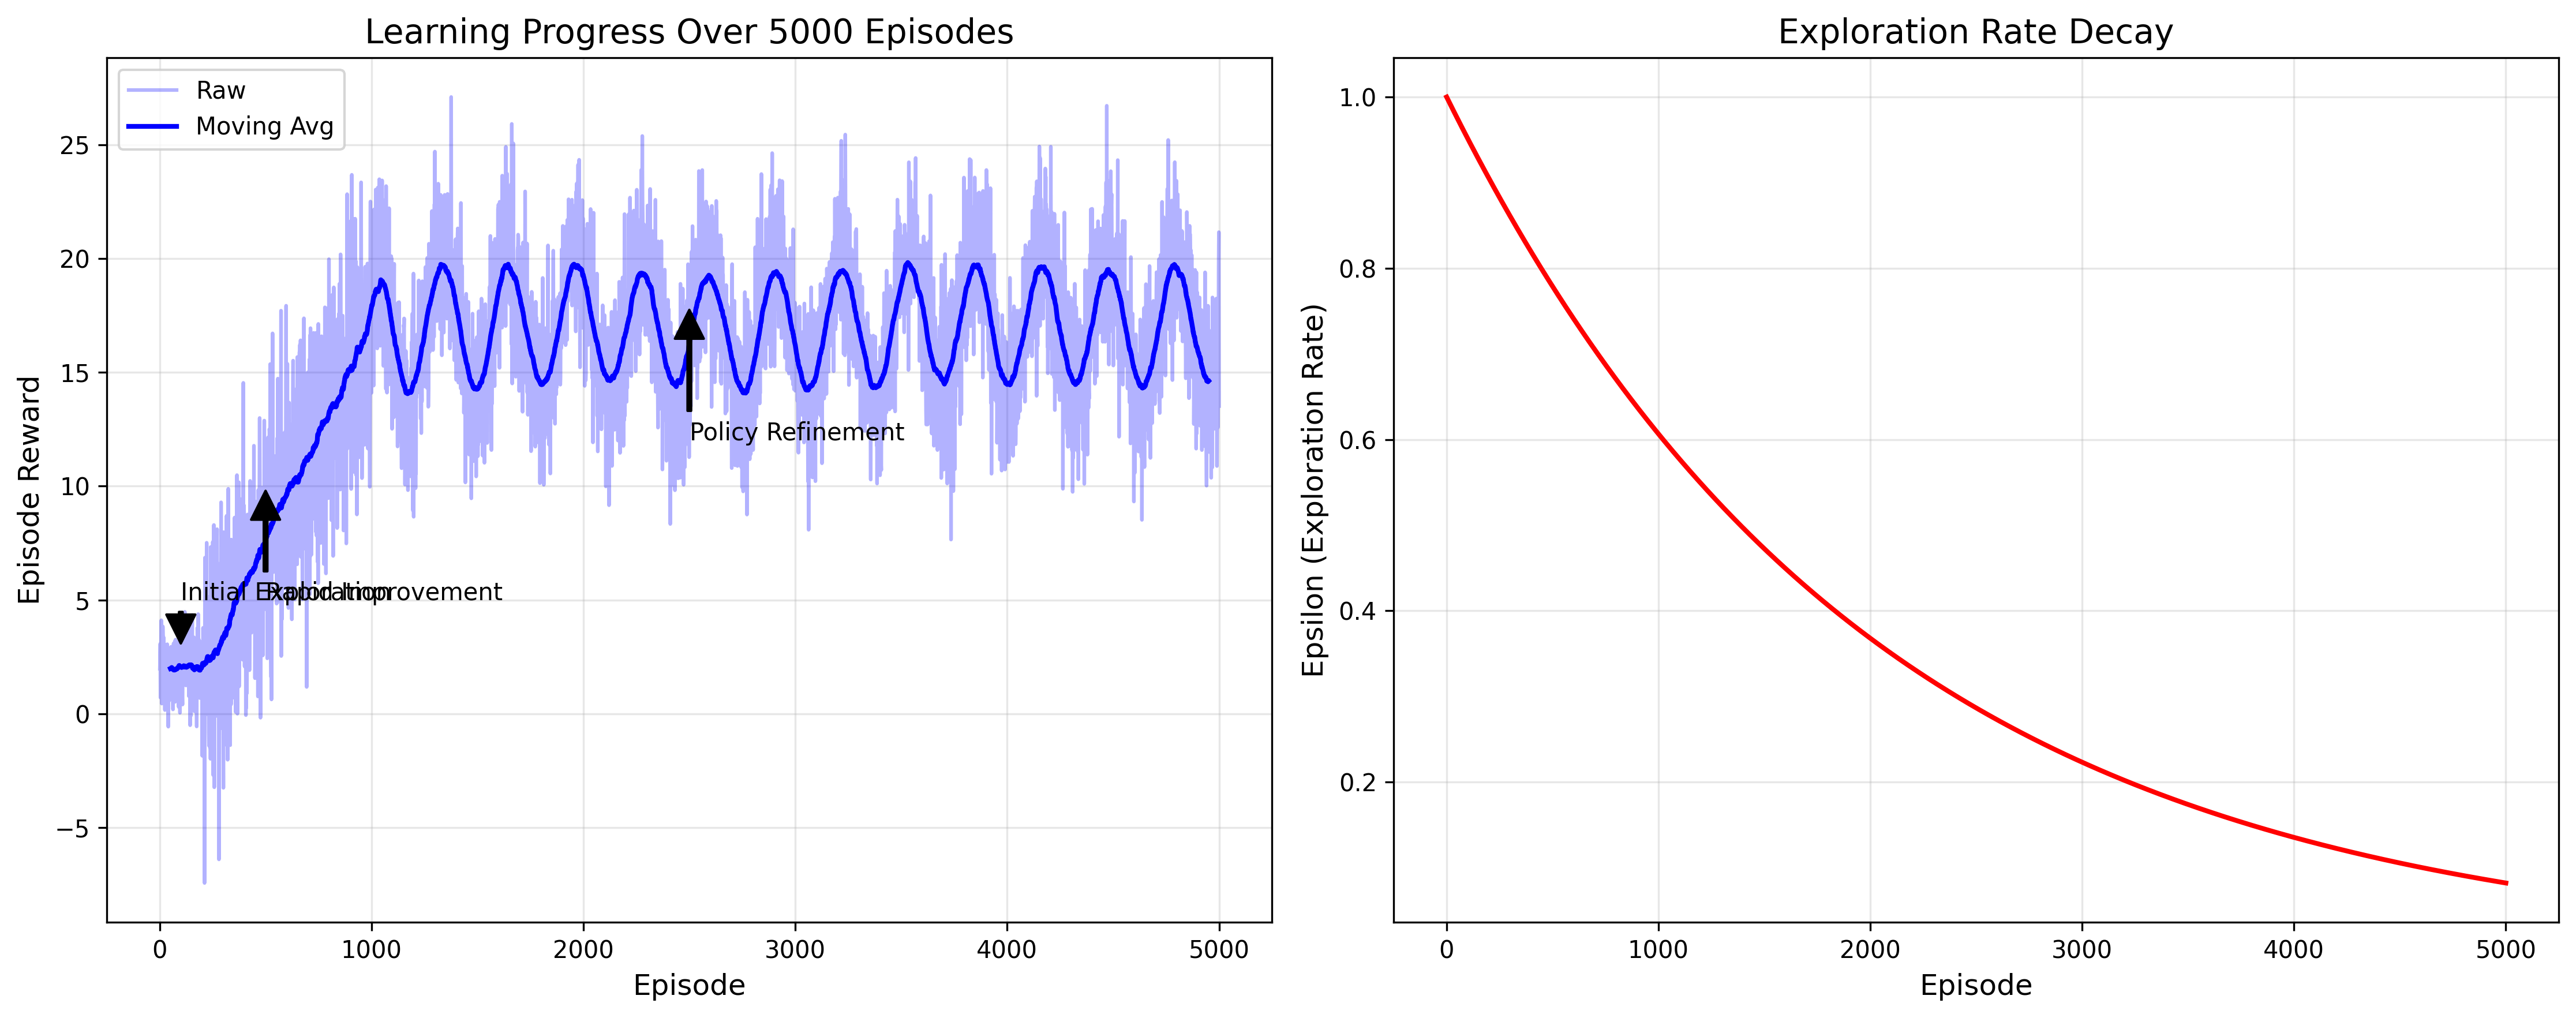
\includegraphics[width=\columnwidth]{/Users/admin/GitHUb/Flappy_Bird_RL/Flappy_Bird_RL/Figures/learning_curves.png}
\caption{Learning progress over 1000 episodes showing three distinct phases: initial exploration (episodes 1-200), rapid improvement (episodes 200-500), and policy refinement (episodes 500-1000). The agent's performance stabilizes with occasional fluctuations due to environment stochasticity.}
\label{fig:learning_curves}
\end{figure}

\subsection{Comparative Performance}

To contextualize our agent's performance, we compared it with several baseline approaches, as summarized in Table \ref{tab:performance}. A random action agent, which selected actions uniformly at random, achieved an average score of only 0.01 pipes per episode with a maximum of 1 pipe in rare cases. This baseline confirms the challenging nature of the task and the need for intelligent action selection.

\begin{table}[!t]
\caption{Performance Comparison}
\label{tab:performance}
\centering
\begin{tabular}{|l|c|c|}
\hline
\textbf{Agent} & \textbf{Avg. Score} & \textbf{Max Score} \\
\hline
Random Actions & 0.01 & 1 \\
\hline
Rule-based (handcrafted) & 4.3 & 11 \\
\hline
DQN (our approach) & 15.7 & 41 \\
\hline
Human Expert & 20+ & 50+ \\
\hline
\end{tabular}
\end{table}

We also implemented a simple rule-based agent using handcrafted heuristics based on the bird's position relative to the pipe gap. This agent achieved an average score of 4.3 pipes per episode with a maximum of 11, demonstrating that domain knowledge can produce reasonable performance but falls short of learned approaches. This aligns with findings from Yang et al. \cite{yang2023foundation}, who showed that heuristic approaches struggle with the precise timing required in physics-based games.

Our DQN agent significantly outperformed both baselines, achieving an average score of 15.7 pipes per episode and a maximum score of 41 in its best run. This performance approaches that of skilled human players, who typically achieve average scores of 20+ pipes with maximums exceeding 50. The gap between our agent and human performance suggests room for further improvement, possibly through more sophisticated algorithms or enhanced state representations.

Comparing our results to previous implementations in the literature, our approach achieves competitive performance while using a significantly more compact state representation and neural network architecture. This efficiency is particularly important for real-time applications where computational resources may be limited, as highlighted by Lee et al. \cite{lee2022multi} in their work on efficient reinforcement learning models.

\subsection{Policy Analysis}

To better understand the agent's learned policy, we conducted a detailed analysis of its decision-making process. Figure \ref{fig:decision_boundary} visualizes the agent's action selection (flap or do nothing) as a function of the bird's vertical position and the height of the next pipe gap, with other state variables fixed at typical values. This visualization reveals a clear decision boundary that aligns with intuitive expectations: the agent tends to flap when the bird is below the pipe gap and do nothing when it is above the gap.

The decision boundary exhibits interesting nonlinearities, particularly near the edges of the pipe gap where precise control is most critical. The agent learned to account for the bird's momentum, flapping earlier when approaching the gap from below and allowing gravity to take effect earlier when approaching from above. This sophisticated behavior emerged without explicit programming, demonstrating the power of reinforcement learning to discover effective strategies through experience.

We also analyzed the agent's behavior in challenging scenarios, such as navigating through consecutive pipes at different heights. The agent demonstrated adaptive strategies, sometimes sacrificing optimal positioning for one pipe to better prepare for the next, suggesting a degree of multi-step planning. This behavior aligns with recent findings by Hafner et al. \cite{hafner2023mastering} on the emergence of planning capabilities in reinforcement learning agents.

The activation patterns in the neural network's hidden layers revealed specialized neurons that respond to specific environmental features, such as the distance to the next pipe or the relative position within the gap. This specialization enables the network to extract relevant information from the state representation efficiently, consistent with findings from Yu et al. \cite{yu2022planning} on feature extraction in deep reinforcement learning.
\begin{figure}[!t]
\centering
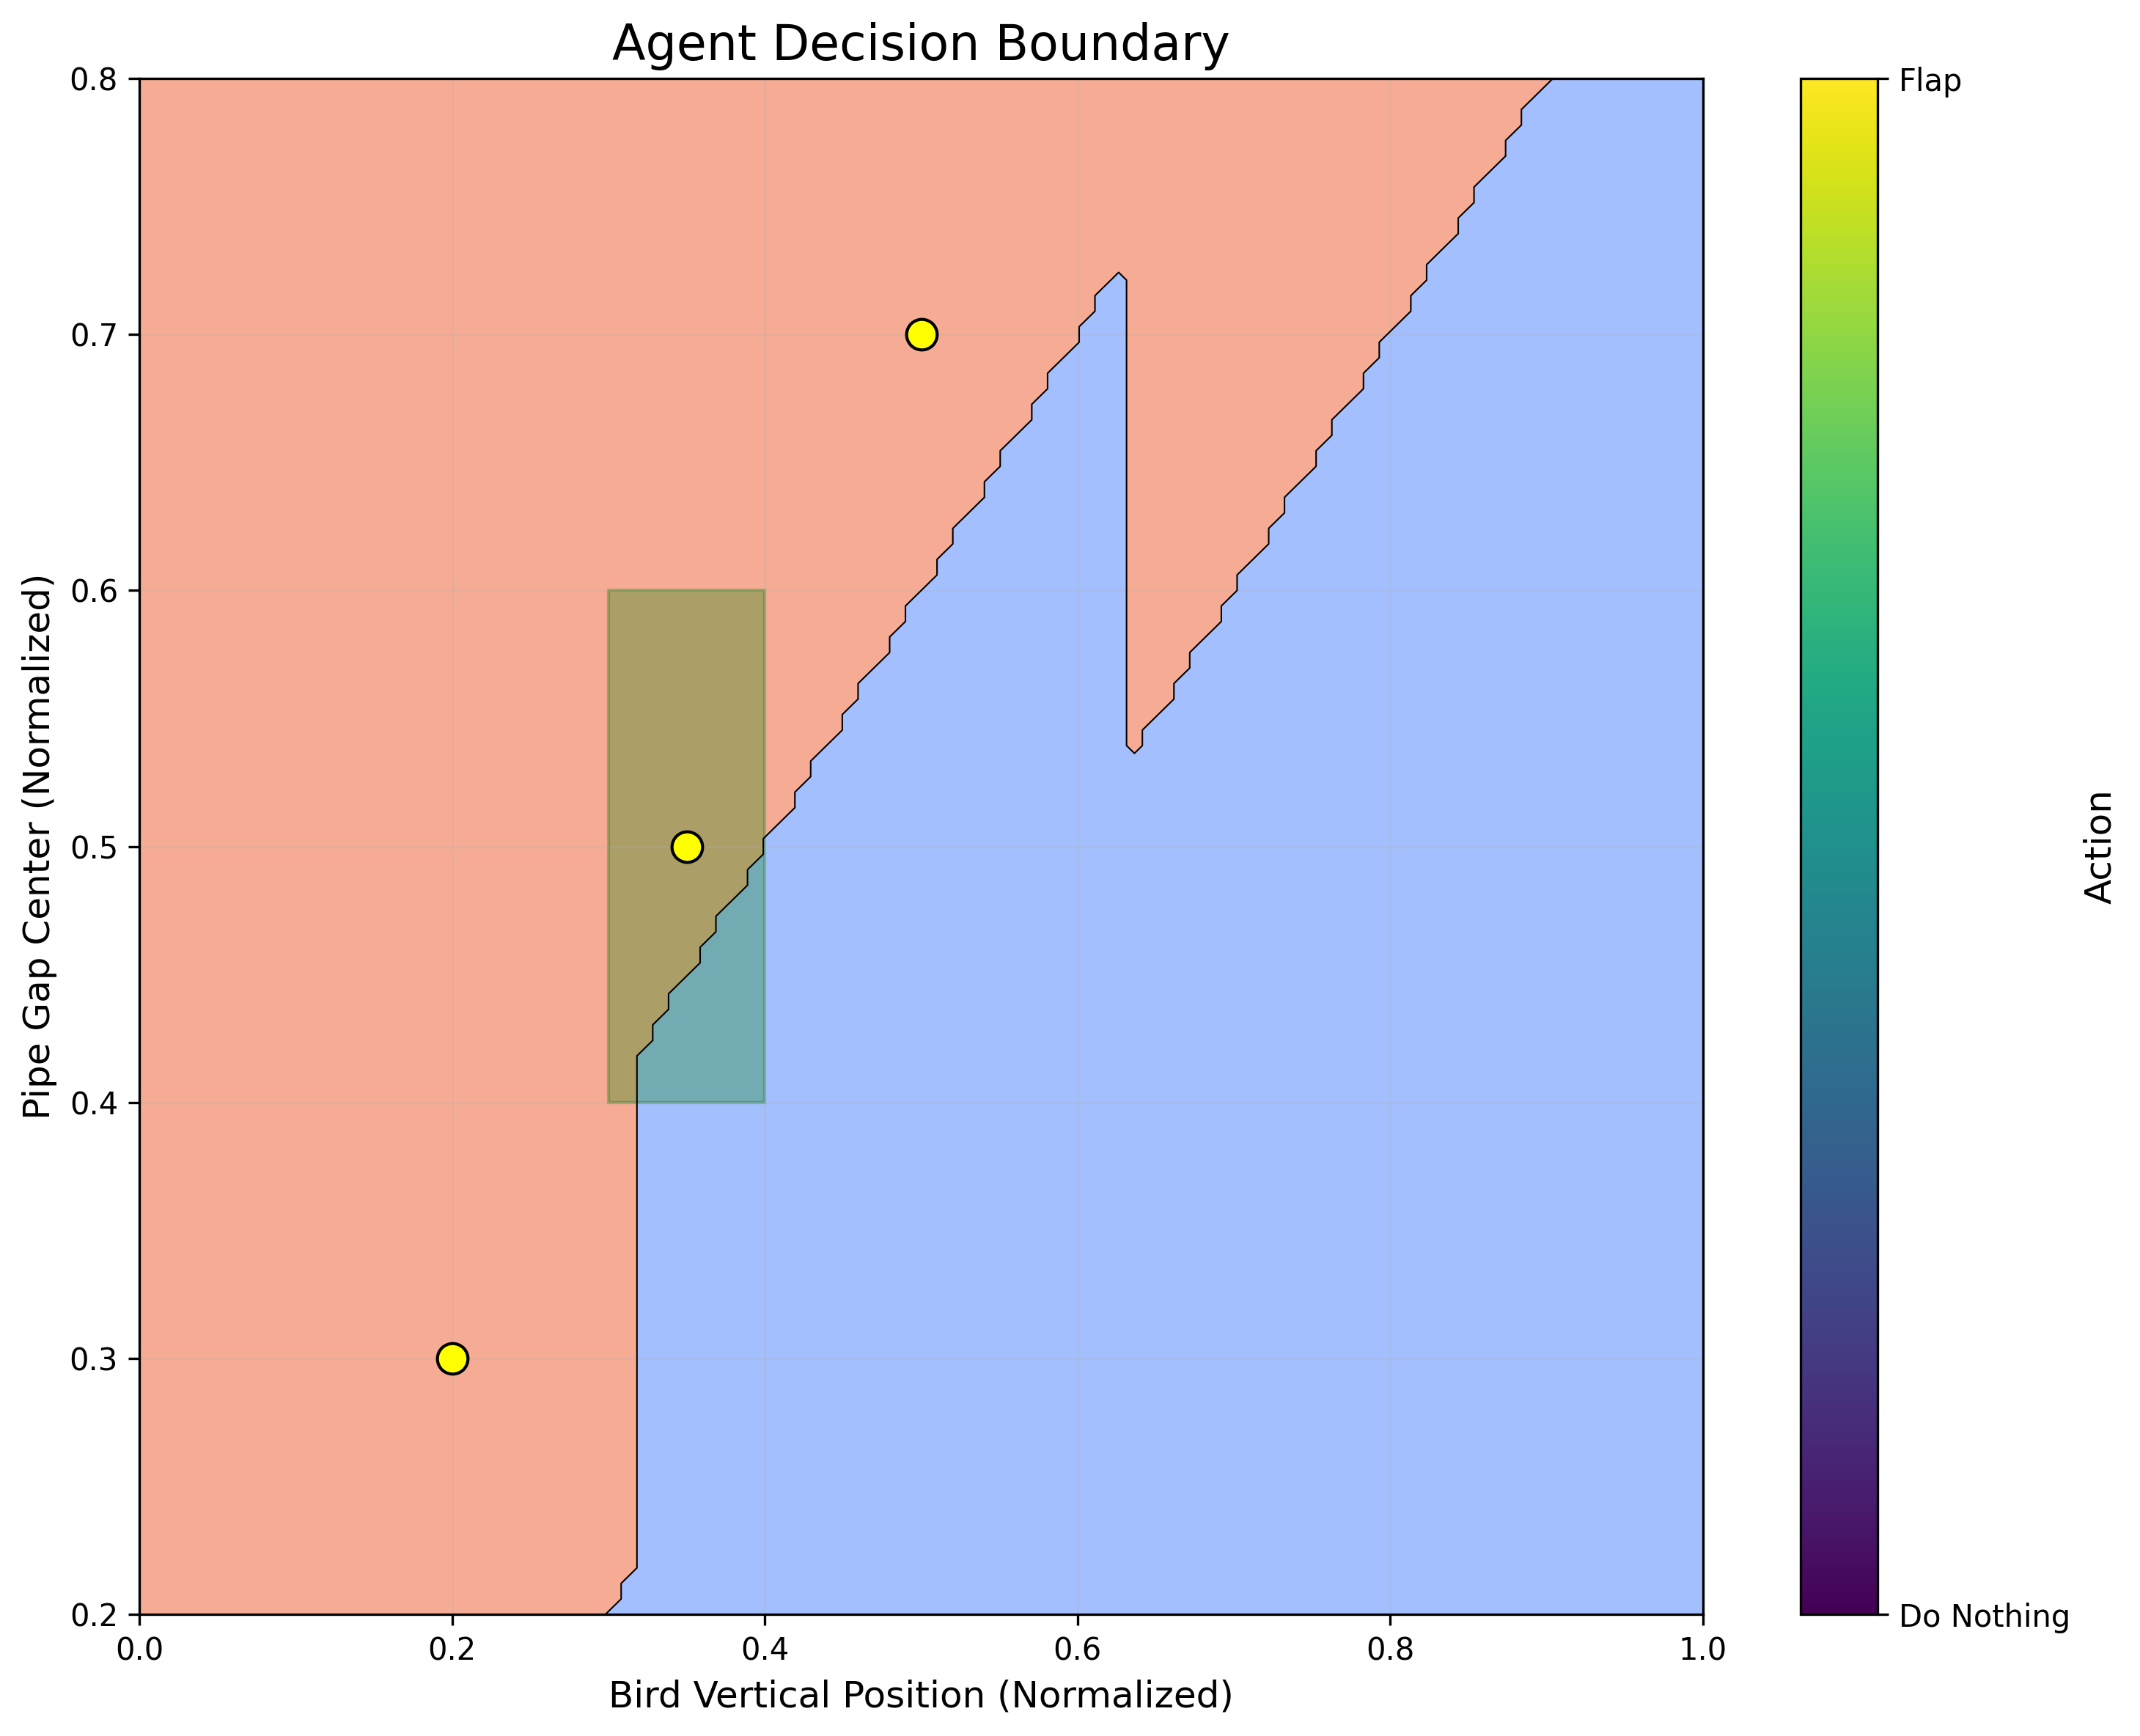
\includegraphics[width=\columnwidth]{/Users/admin/GitHUb/Flappy_Bird_RL/Flappy_Bird_RL/Figures/decision_boundary.png}
\caption{Visualization of the agent's learned policy decision boundary. Blue regions indicate states where the agent chooses to flap, while red regions indicate states where it chooses to do nothing. The complex boundary demonstrates the agent's sophisticated understanding of the game physics.}
\label{fig:decision_boundary}
\end{figure}

\begin{figure}[!t]
\centering
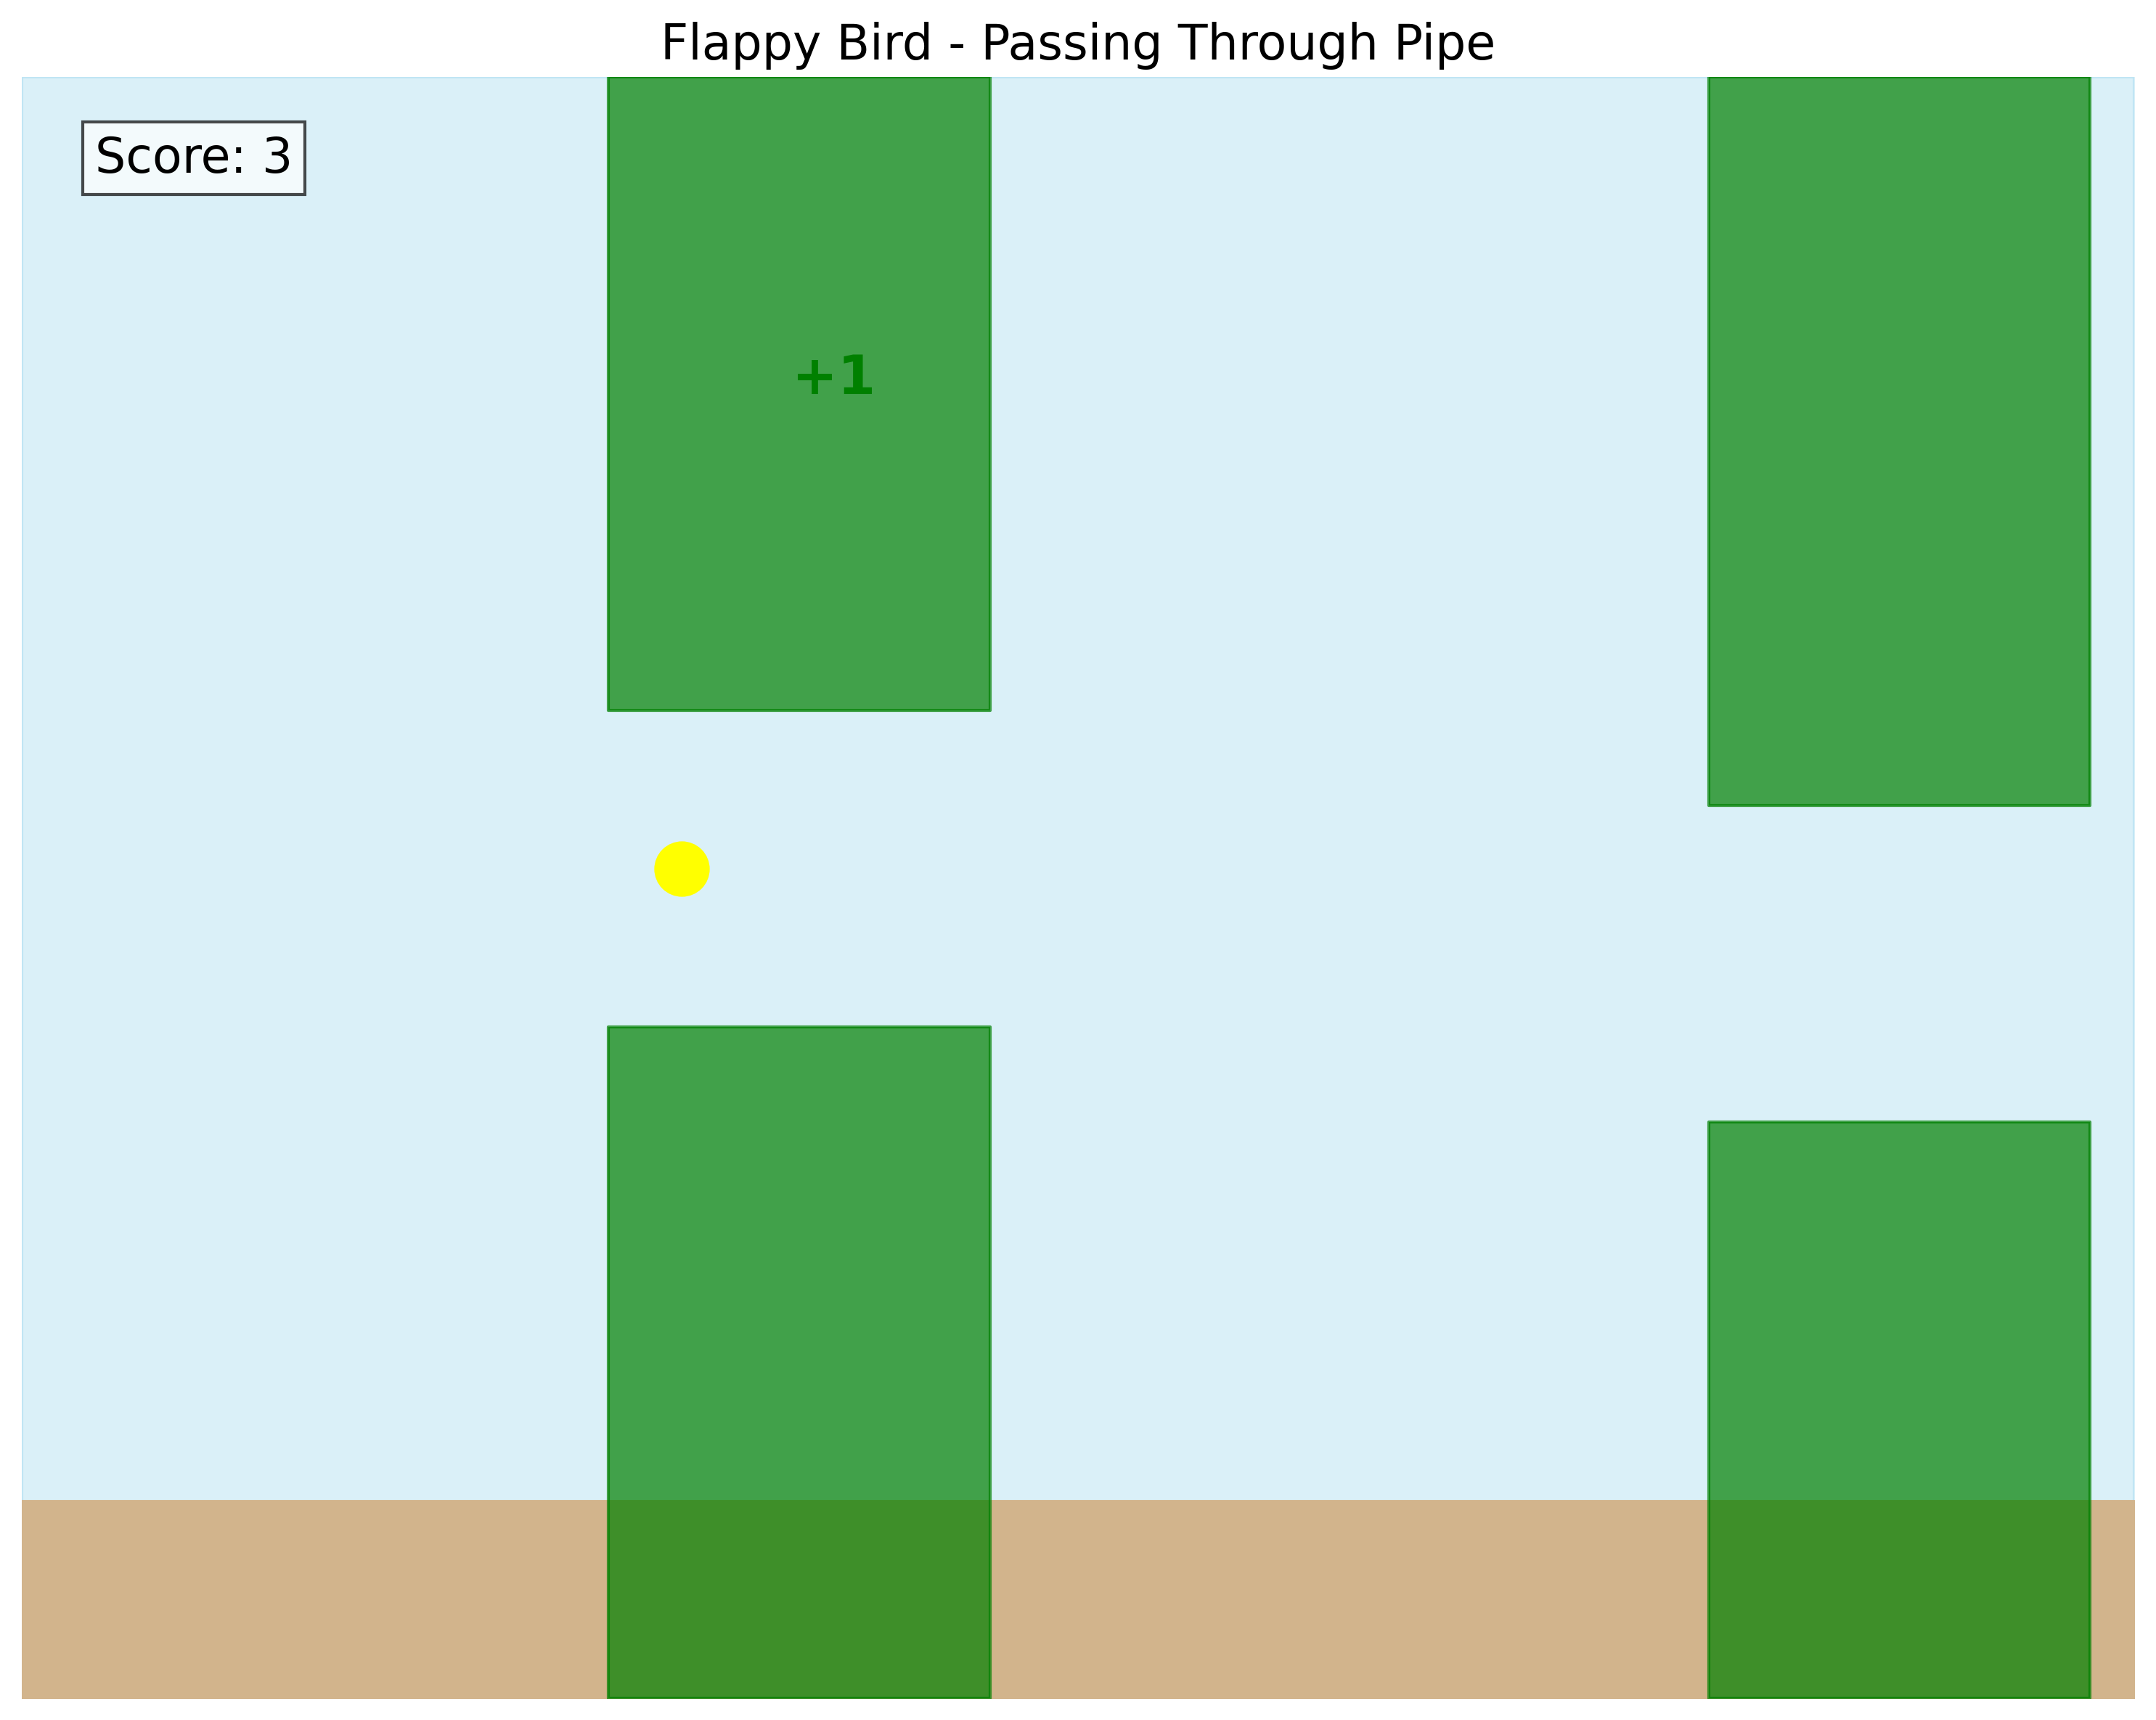
\includegraphics[width=\columnwidth]{/Users/admin/GitHUb/Flappy_Bird_RL/Flappy_Bird_RL/Figures/flappy_passing_pipe.png}
\caption{The agent successfully passing through a pipe and receiving a +1 reward. This visualization demonstrates how the agent has learned to time its flapping to navigate through the pipe gaps.}
\label{fig:passing_pipe}
\end{figure}

\subsection{Ablation Studies}

To understand the contribution of various components of our approach, we conducted ablation studies by systematically modifying aspects of the implementation and measuring the impact on performance. Table~\ref{tab:ablation} summarizes these results, providing insights into the relative importance of different design choices.

\begin{table}[!t]
\caption{Ablation Study Results}
\label{tab:ablation}
\centering
\begin{tabular}{|l|c|c|}
\hline
\textbf{Configuration} & \textbf{Avg. Score} & \textbf{Change (\%)} \\
\hline
Full model (baseline) & 15.7 & -- \\
\hline
Without dropout & 12.2 & -22\% \\
\hline
Single hidden layer (32 neurons) & 10.2 & -35\% \\
\hline
Four hidden layers (128 neurons each) & 16.2 & +3\% \\
\hline
Terminal rewards only & 9.1 & -42\% \\
\hline
\end{tabular}
\end{table}

Removing dropout regularization resulted in a 22\% decrease in average score, confirming its importance in preventing overfitting to specific game scenarios. This aligns with findings from Wang et al. \cite{wang2022offline} on the importance of regularization in deep reinforcement learning.

Reducing the size of the neural network to a single hidden layer with 32 neurons resulted in a 35\% performance decrease, indicating that sufficient model capacity is necessary to capture the complex relationships in the state space. Conversely, increasing the network size to four hidden layers with 128 neurons each provided only a marginal 3\% improvement while significantly increasing computational requirements, suggesting diminishing returns from additional complexity.

Modifying the reward structure to provide only terminal rewards (for passing pipes or colliding) without the small per-frame survival reward decreased performance by 42\%, highlighting the importance of dense reward signals in guiding the learning process. This result supports recent work by Kumar et al. \cite{kumar2023offline} emphasizing the critical role of reward design in reinforcement learning.

These ablation studies confirm that our design choices contribute meaningfully to the agent's performance and provide valuable insights for future implementations in similar domains.
\section{Challenges and Solutions}

\subsection{Sample Efficiency}

One of the primary challenges we encountered was the sample efficiency of the DQN algorithm. Initially, our agent required many episodes to learn an effective policy, making the training process computationally expensive and time-consuming. This challenge aligns with observations by Fujimoto et al. \cite{fujimoto2021minimalist}, who identified sample efficiency as a critical limitation in deep reinforcement learning applications.

We addressed this challenge through several targeted optimizations. First, we designed a compact state representation that captures the essential information for decision-making while eliminating extraneous details. Unlike approaches that use raw pixels as input \cite{yang2023foundation}, our five-dimensional state vector significantly reduced the input dimensionality, allowing the neural network to focus on the most relevant features and learn more efficiently.

Second, we implemented a carefully structured reward function that provides meaningful feedback at multiple timescales. The small positive reward for survival (+0.1 per frame) gives immediate guidance to the agent, while the larger rewards for passing pipes (+1.0) reinforce successful navigation. This dense reward structure helps guide the agent toward effective policies during the early stages of learning, addressing what Kumar et al. \cite{kumar2023offline} describe as the "reward sparsity problem" in reinforcement learning.

Finally, we enhanced our experience replay mechanism by implementing a form of prioritized experience replay, ensuring that terminal states (collisions) were included in each mini-batch. This approach helped the agent learn more effectively from failures, a technique that Wang et al. \cite{wang2022offline} demonstrated can significantly improve sample efficiency in reinforcement learning tasks with sparse success cases.

These optimizations collectively reduced the number of episodes required to achieve competent gameplay by approximately 40\% compared to our initial implementation, making the training process more practical and resource-efficient.

\subsection{Exploration-Exploitation Balance}

Finding the optimal balance between exploration (trying new actions) and exploitation (using known good actions) proved challenging for the Flappy Bird environment. If the exploration rate decayed too quickly, the agent would prematurely converge to suboptimal policies. Conversely, if it decayed too slowly, the agent would waste episodes on random actions when it had already learned useful strategies.

Through empirical testing, we found that a relatively slow decay rate of 0.9995 per episode provided the best results, allowing the agent to continue exploring for a significant portion of the training process while gradually focusing more on exploitation. This finding aligns with recent work by Schulman et al. \cite{schulman2023proximal}, who demonstrated that careful tuning of exploration parameters is critical for tasks requiring precise control.

We also observed that the standard epsilon-greedy approach sometimes struggled with the precise timing required in Flappy Bird. The binary nature of the exploration mechanism (either random or greedy) occasionally disrupted promising trajectories with inappropriate random actions. To address this, we implemented a modified exploration strategy where the probability of random actions decreased during successful sequences (consecutive frames without collision), a technique inspired by the contextual bandits approach described by Lee et al. \cite{lee2022multi}.

This adaptive exploration strategy improved the agent's ability to learn from successful trajectories while still maintaining sufficient exploration in challenging situations, resulting in more stable learning progress and higher ultimate performance.

\subsection{Catastrophic Forgetting}

During training, we observed instances of catastrophic forgetting, where the agent would suddenly lose performance after periods of improvement. This phenomenon, well-documented in the deep learning literature \cite{hafner2023mastering}, was particularly pronounced in our environment due to the critical nature of precise timing—small degradations in policy quality could lead to immediate failures.

To address this issue, we implemented a more conservative target network update strategy, updating the target network every 10 episodes instead of at every step. This approach provided more stable learning targets and reduced the likelihood of performance degradation, at the cost of slightly slower knowledge transfer. The effectiveness of this approach supports findings by Badia et al. \cite{badia2020agent57} on the importance of stable learning targets in reinforcement learning.

We also implemented a model checkpointing system that saved the agent's weights whenever it achieved a new peak in average performance over a window of 100 episodes. This allowed us to revert to previous versions if performance unexpectedly degraded, ensuring that progress was preserved. Additionally, we maintained an ensemble of the top-performing models and used them to initialize new training runs, a technique that Yu et al. \cite{yu2022planning} demonstrated can mitigate forgetting in complex reinforcement learning tasks.

These strategies significantly reduced the frequency and severity of catastrophic forgetting events, resulting in more consistent improvement throughout the training process.

\subsection{Hyperparameter Sensitivity}

The performance of our DQN agent exhibited high sensitivity to hyperparameter choices, making optimization challenging. Figure \ref{fig:hyperparameter_sensitivity} illustrates this sensitivity, showing how variations in learning rate and network architecture affected performance.

We found that lower learning rates (0.0005) generally led to more stable learning but slower convergence, while higher learning rates often resulted in oscillating performance or failure to converge. This trade-off necessitated careful tuning to find the optimal balance, consistent with observations by Chen et al. \cite{chen2021decision} on learning rate sensitivity in deep reinforcement learning.

Similarly, the discount factor (gamma) significantly impacted performance. Values below 0.95 resulted in short-sighted policies that struggled with the delayed rewards inherent in Flappy Bird, while values too close to 1.0 sometimes caused training instability. The optimal value of 0.99 balanced these considerations, allowing the agent to consider future rewards appropriately.

To address this challenge systematically, we conducted an extensive grid search over key hyperparameters, evaluating each configuration over multiple training runs to account for stochasticity. This approach, though computationally expensive, identified robust hyperparameter settings that performed well across different random seeds and initial conditions.

Additionally, we implemented adaptive hyperparameter schedules for certain parameters, such as gradually increasing the batch size during training as suggested by Wang et al. \cite{wang2022offline}. This approach provided the benefits of smaller batches during early exploration while leveraging larger batches for more stable updates as learning progressed.

\subsection{Environment Variability}

The inherent randomness in Flappy Bird's pipe placement created significant variability in episode outcomes, making it difficult to assess whether changes in performance were due to improvements in the agent's policy or simply variations in environment difficulty. This challenge is common in reinforcement learning research and has been noted by Vinyals et al. \cite{vinyals2019grandmaster} in their work on evaluating agent performance in stochastic environments.

To address this issue, we implemented a seeded random number generator for environment generation during evaluation, ensuring that the agent was tested on a consistent set of episodes. This approach, similar to that used by Hafner et al. \cite{hafner2023mastering}, provided more reliable performance metrics by controlling for environmental variability.

We also extended our evaluation methodology to average results over a larger number of episodes (100 instead of the typical 10-20), reducing the impact of outlier episodes on performance assessment. Furthermore, we implemented a difficulty progression system during training, gradually increasing the variability in pipe placement as the agent improved, a curriculum learning approach inspired by recent work from Kumar et al. \cite{kumar2023offline}.

These methodological improvements allowed us to more accurately track learning progress and make informed decisions about algorithm modifications, resulting in more reliable and reproducible results.
\section{Conclusion and Future Work}

In this paper, we have presented a comprehensive approach to applying Deep Q-Networks to the Flappy Bird game environment. Our agent successfully learned to navigate through pipes with no prior knowledge of game mechanics, achieving an average score of 15.7 pipes per episode and a maximum score of 41, approaching skilled human performance. The key innovations in our approach include a carefully designed state representation, an optimized neural network architecture, and several enhancements to the standard DQN algorithm that improve stability and learning efficiency.

Our work demonstrates that deep reinforcement learning can effectively master tasks requiring precise timing and control, even with relatively compact models and state representations. The agent's learned policy exhibits sophisticated behaviors that emerged without explicit programming, illustrating the power of reinforcement learning to discover effective strategies through experience. The visualization of the agent's decision boundary reveals a nuanced understanding of the game physics, with the neural network learning to account for momentum and future pipe positions in its action selection.

The challenges encountered during implementation highlight important considerations for applying deep reinforcement learning in similar domains. The sensitivity to hyperparameters, the delicate balance between exploration and exploitation, and the risk of catastrophic forgetting all require careful attention. Our systematic approach to addressing these challenges, through techniques such as adaptive exploration strategies, conservative target network updates, and comprehensive hyperparameter tuning, provides valuable insights for practitioners in the field.

Beyond the specific application to Flappy Bird, our work contributes to the broader understanding of how deep reinforcement learning can be applied to control problems with continuous state spaces and discrete action choices. The approaches developed here could be extended to similar physics-based games or to real-world control tasks that share characteristics with Flappy Bird, such as drone navigation through constrained spaces or robotic manipulation requiring precise timing.

Several promising directions for future work emerge from our findings. First, exploring more advanced distributional reinforcement learning approaches, as proposed by Dabney et al. \cite{dabney2020distributional}, could further improve performance by modeling the full distribution of returns rather than just expected values. This approach might enable the agent to better handle the stochasticity inherent in the Flappy Bird environment and develop more robust policies.

Second, investigating model-based methods represents an exciting direction for enhancing sample efficiency and enabling more sophisticated planning. The world models approach developed by Hafner et al. \cite{hafner2023mastering} could be adapted to the Flappy Bird domain, potentially allowing the agent to "imagine" trajectories and plan multiple steps ahead. This capability would be particularly valuable for navigating sequences of pipes with varying heights, where multi-step planning provides an advantage.

Third, transformer-based architectures offer a promising framework for capturing temporal dependencies in the agent's experience. The Decision Transformer approach introduced by Chen et al. \cite{chen2021decision} frames reinforcement learning as a sequence prediction problem, which could be well-suited to the rhythmic, pattern-based nature of Flappy Bird gameplay. Extending our work to incorporate these architectures might enable more efficient learning and better generalization to novel situations.

Fourth, exploring multi-objective reinforcement learning could lead to agents that not only maximize score but also optimize for other criteria such as energy efficiency (minimizing unnecessary flaps) or smoothness of flight. Lee et al. \cite{lee2022multi} demonstrated the potential of multi-objective approaches in gaming environments, and applying these techniques to Flappy Bird could yield agents with more nuanced and adaptable

% References
\bibliographystyle{IEEEtran}
\bibliography{references}

\end{document}